% main.tex -- International Journal of Remote Sensing manuscript

\documentclass[]{interact}
\usepackage{epstopdf}% To incorporate .eps illustrations using PDFLaTeX, etc.
\usepackage[caption=false]{subfig}% Support for small, `sub' figures and tables
%\usepackage[nolists,tablesfirst]{endfloat}% To `separate' figures and tables from text if required
%\usepackage[doublespacing]{setspace}% To produce a `double spaced' document if required
%\setlength\parindent{24pt}% To increase paragraph indentation when line spacing is doubled

%\usepackage[numbers,sort]{natbib}% Citation support using natbib.sty (numbered P style)
%\bibpunct[, ]{(}{)}{;}{n}{,}{,}% Citation support using natbib.sty (numeric mode)
%\renewcommand\bibfont{\fontsize{10}{12}\selectfont}% To set the list of references in 10 point font using natbib.sty
\usepackage[natbibapa]{apacite}% APA author-year citation support. Commands using natbib.sty MUST be deactivated first!
\setlength\bibhang{12pt}% To set the indentation in the list of references using apacite.sty.
\renewcommand\bibliographytypesize{\fontsize{10}{12}\selectfont}% To set the list of references in 10 point font using apacite.sty.
\usepackage[colorlinks=true, citecolor=blue, linkcolor=blue, urlcolor=blue]{hyperref}% Clickable hyperlinks


\theoremstyle{plain}% Theorem-like structures provided by amsthm.sty
\newtheorem{theorem}{Theorem}[section]
\newtheorem{lemma}[theorem]{Lemma}
\newtheorem{corollary}[theorem]{Corollary}
\newtheorem{proposition}[theorem]{Proposition}

\theoremstyle{definition}
\newtheorem{definition}[theorem]{Definition}
\newtheorem{example}[theorem]{Example}

\theoremstyle{remark}
\newtheorem{remark}{Remark}
\newtheorem{notation}{Notation}

\begin{document}

\articletype{Review Article}% Specify the article type or omit as appropriate

\title{Deep learning and multi-level fusion for land-use and land-cover classification: Technological evolution trajectory and future trends}

\author{
\name{Jie Cheng\textsuperscript{a}, Jie Xie\textsuperscript{a}\thanks{CONTACT Jie Xie. Email: xiej8734@gmail.com}, Shupei Xia\textsuperscript{a} and Alejandro C.\ Frery\textsuperscript{b}}
\affil{\textsuperscript{a}School of Computer and Electronic Information / School of Artificial Intelligence, Nanjing Normal University, Nanjing, China; \textsuperscript{b}School of Mathematics and Statistics, Victoria University of Wellington, New Zealand}
}

\maketitle

\begin{abstract}
Land Use/Land Cover Change (LULCC) is essential to understand human-environment interactions, ecological impacts, and sustainable land management. Given the growing complexity and scale of LULCC dynamics, accurately capturing these processes remains a significant challenge. With the development of earth observation technology and artificial intelligence, deep learning combined with multi-source data fusion has become the core driving force for the LULCC simulation. To clarify the trajectory of technological evolution and future trends in this field, this study conducts an in-depth analysis of 261 core literatures published from 2006 to 2025 based on the Web of Science Core Collection, integrating systematic and bibliometric review methods. Our results show that: (1) The number of published papers in this field has witnessed an exponential growth since 2016; (2) In terms of technological paradigms, the research focus has undergone a fundamental shift from single data source and traditional machine learning to multi-source heterogeneous data fusion and deep learning; (3) Feature-level fusion has replaced data-level and decision-level fusion as the current main strategy; (4) Future research should focus on the development of Explainable Artificial Intelligence, general remote sensing foundation models, and intelligent data governance technologies.
\end{abstract}

\begin{keywords}
Land Use/Land Cover, Deep Learning, Multi-source Data Fusion, Feature Fusion, Transformer, Mamba
\end{keywords}


\section{Introduction}

Land-use and land-cover (LULC) information constitutes a fundamental baseline for understanding Earth system dynamics and is pivotal in urban planning, ecosystem assessment, disaster monitoring, and global climate change research \citep{ORIG1}. However, optical remote sensing alone is insufficient to capture the full complexity of land surface processes. Consequently, complementary modalities including LiDAR, SAR, and GNSS are increasingly essential, as they provide unique structural, temporal, and positional information. With the rapid advancement of Earth observation technologies that integrate these multi-source data, the field has entered the era of remote sensing big data, characterized by high spatial, temporal, and hyperspectral resolutions. Nonetheless, accurate and automated classification of complex Earth surface dynamics remains a significant challenge in geographic information science.


Historically, LULC classification initially relied on statistical methods such as Gaussian maximum likelihood classification and later shifted to traditional machine learning algorithms like Support Vector Machines (SVM) and Random Forest (RF). While effective for small-scale areas, these shallow models often fail to capture high-level semantic features and depend substantially on manual feature engineering, which consequently limits their generalization capabilities in complex heterogeneous scenes. Since 2015, the emergence of Deep Learning (DL) has substantially transformed the field \citep{2}. Algorithms including Convolutional Neural Network (CNN) and the more recent Transformer have consistently outperformed traditional methods by automatically learning hierarchical representations directly from raw data.



Parallel to the evolution of algorithms, the limitations of single-source remote sensing data have become increasingly prominent. Optical imagery is susceptible to cloud cover and lighting conditions, SAR lacks rich spectral information, and LiDAR data is often constrained by acquisition costs. Consequently, multi-source data fusion that integrates the complementary strengths of optical imagery in terms of spectral content, SAR with respect to texture, structure, and dielectric properties, and LiDAR for elevation information has become an inevitable strategy to overcome the accuracy limitations of LULC classification. The intersection of deep learning and multi-source fusion now represents the current technical frontier. Despite the exponential growth in publications, a comprehensive understanding of how these technologies have evolved over the past two decades remains relatively fragmented \citep{5}.





Although numerous review articles on LULC classification or remote sensing data fusion have been published, existing studies face several limitations in meeting the demand for a macro-scale understanding of the field's evolution. First, existing reviews often focus on a single technical lineage and suffer from a time lag. For instance, Ma et al. systematically summarized the early applications of deep learning in remote sensing, but their focus was primarily on CNN architectures \citep{ORIGma2019deep}. Since their work predates the emergence of Vision Foundation Models such as Transformer and State Space Models like Mamba after 2020, it fails to cover the latest technical paradigm shifts. While recent scholars including Aleissaee et al. have provided specialized reviews on Transformers, they concentrate on emerging technologies with limited discussion of previous traditional algorithms \citep{7}. Second, there is a lack of quantitative scientometric support. Although Ghamisi et al. provided a detailed technical categorization of multi-source data fusion strategies including data-level, feature-level, and decision-level fusion, their work remains a qualitative technical review \citep{ORIG6,7,8}. Such articles tend to list algorithmic details without the support of large-sample bibliometric analysis, making it difficult for researchers to objectively grasp the geographical distribution of global research power, the evolution of collaboration networks, and the spatio-temporal migration of research hotspots from a macro perspective.



This study conducts a systematic bibliometric analysis and review based on the Web of Science Core Collection for the period 2006--2025. Unlike previous studies that focus solely on algorithmic techniques or traditional reviews, this paper combines quantitative bibliometric indicators (utilizing tools such as VOSviewer and HistCite \citep{9,10}) with qualitative technical discussions. This research aims to: (1) map the global research landscape to identify core countries, institutions, and high-impact authors; (2) track the evolution of research hotspots, particularly the shift from CNN-based feature extraction to emerging trends such as Transformer and attention mechanisms; (3) compare the effectiveness of different fusion strategies, highlighting the dominance of feature fusion; and (4) critically analyze current challenges (e.g., data heterogeneity and model interpretability) to explore potential future research trajectories \citep{ORIGli2024feddiff}.

\section{Data and Methods}

\subsection{Data Collection}
\label{sec:data_collection} 
In the contemporary era, scientific literature datasets have become increasingly accessible to researchers. The Web of Science (WoS) is widely recognized as one of the most authoritative and representative scientific databases globally. Therefore, the data utilized for this review were primarily retrieved from the WoS Core Collection \citep{11}. To comprehensively cover various models and simulation studies related to LULC, and to clearly define the research scope of the field, the search query was constructed and is summarized in Table~\ref{tab:search_strategy}. 

Considering that deep learning has emerged as a relatively recent research hotspot, the time span was set from 2006 to 2025 to capture pivotal progress in LULC modeling. During the early 21st century, major global environmental initiatives were dominated by traditional methodologies; however, the subsequent surge in deep learning has fundamentally reshaped the field's methodological landscape. The final retrieval, completed in December 2025, yielded a total of 261 relevant publications. The detailed classification and statistics of the search results are summarized in Table~\ref{tab:search_strategy}.


\begin{table}[htb!]
	\centering
	\setlength{\belowcaptionskip}{5pt}
	\caption{Detailed classification and statistics of the literature search strategy.}
	\label{tab:search_strategy}
	\small 
	\renewcommand{\arraystretch}{1.4}
	\begin{tabular}{@{} p{4.5cm} p{10cm} @{}} 
		\toprule
		\textbf{Item} & \textbf{Details} \\
		\midrule
		Data source & Web of Science Core Collection \\
		Period & 2006--2025 \\
		Language & English \\
		Document type & ``Article'', ``Proceeding Paper'' \\
		Search date & December 2025 \\
		\midrule
		\textbf{Search structure} & \textbf{(Three conceptual blocks, combined with AND)} \\
		Block A (sensor/method) & ``ensemble'' OR ``fusion'' \\
		Block B (topic) & ``land use classification'' OR ``land cover classification'' OR ``land use recognition'' OR ``land cover recognition'' OR ``land use detection'' OR ``land cover detection'' \\
		Block C (technique) & ``deep learning'' \\
		\midrule
		Full Boolean query & \parbox{10cm}{\texttt{(``ensemble'' OR ``fusion'') AND (``land use classification'' OR ``land cover classification'' OR ``land use recognition'' OR ``land cover recognition'' OR ``land use detection'' OR ``land cover detection'') AND (``deep learning'')}} \\
		\bottomrule
	\end{tabular}
\end{table}


\subsection{Research Framework and Methodology}
\label{sec:methodology}

The research framework of this study is structured into three distinct phases: data collection, bibliometric analysis, and discussion/synthesis, as illustrated in Fig.~\ref{fig:flowchart}. 

During the data collection phase, literature retrieval was conducted using the advanced search function within the Web of Science Core Collection, with the specific search strategy detailed in Section~\ref{sec:data_collection}. An initial screening was performed based on language (limited to English) and document type (excluding Review Articles, Early Access, Retracted Publications, and Editorial Material). This resulted in a final dataset of 261 relevant publications. These rigorous inclusion criteria ensure a high-quality sample library based on peer-reviewed research. Notably, Review Articles were excluded to avoid potential ``noise'' or over-representation in citation analysis, as they typically cite a vast number of papers. Other document types were omitted due to their limited quantity and lower thematic relevance. Consequently, ``Articles'' and ``Proceeding Papers'' were selected as the primary document types for this study \citep{ORIG12}.

This study combines fundamental bibliometric analysis \citep{14,16} with network analysis methods \citep{13} to reveal global academic trends and identify research hotspots in the field of LULC remote sensing classification. For a better understanding of the subsequent analysis, the relevant numerical indicators are introduced first, followed by an elaboration on network-based analysis methods, including co-word analysis, co-author analysis, and co-citation analysis. 




Currently, several software tools are available for the analysis and visualization of scientometric information. In this study, three specialized tools were employed: HistCite, VOSviewer, and the Bibliometrix R package \citep{15}. HistCite provides a highly functional interactive interface capable of outputting diverse statistical metrics, such as annual publication volume and rankings of representative authors, countries, journals, and institutions \citep{9}. Bibliometrix and VOSviewer were utilized to construct and comprehensively analyze co-word networks \citep{17}, co-author relationships \citep{18}, and co-citation references \citep{19}.



The annual publication output reflects the research activity and academic influence within a specific field over time. In this study, we explore the status of LULC classification research by analyzing the temporal distribution of annual publications, Total Local Citation Score (TLCS), and Total Global Citation Score (TGCS) \citep{20}. While the number of publications directly represents the volume of records indexed in the Web of Science database each year, TLCS and TGCS measure the local and global academic impact of these works, respectively. The trends for LULC research from 2016 to 2025 are illustrated in Fig.~\ref{fig:pub_trends}.

\begin{figure}[htb!]
	\centering
	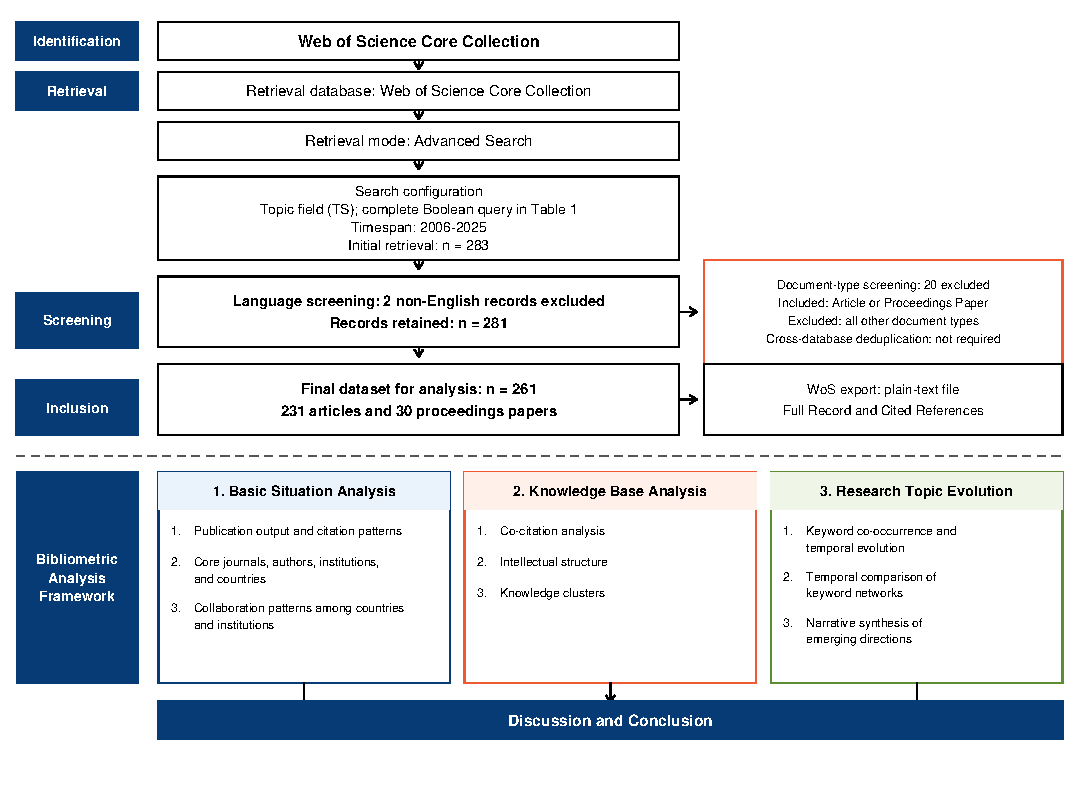
\includegraphics[width=0.9\linewidth]{Figures/flowchart.pdf} 
	\caption{Flowchart of the research on technological development in LULC.}
	\label{fig:flowchart}
\end{figure}


\section{Basic Situation Analysis}
\subsection{Yearly Output}

\begin{figure}[htb!]
	\centering
	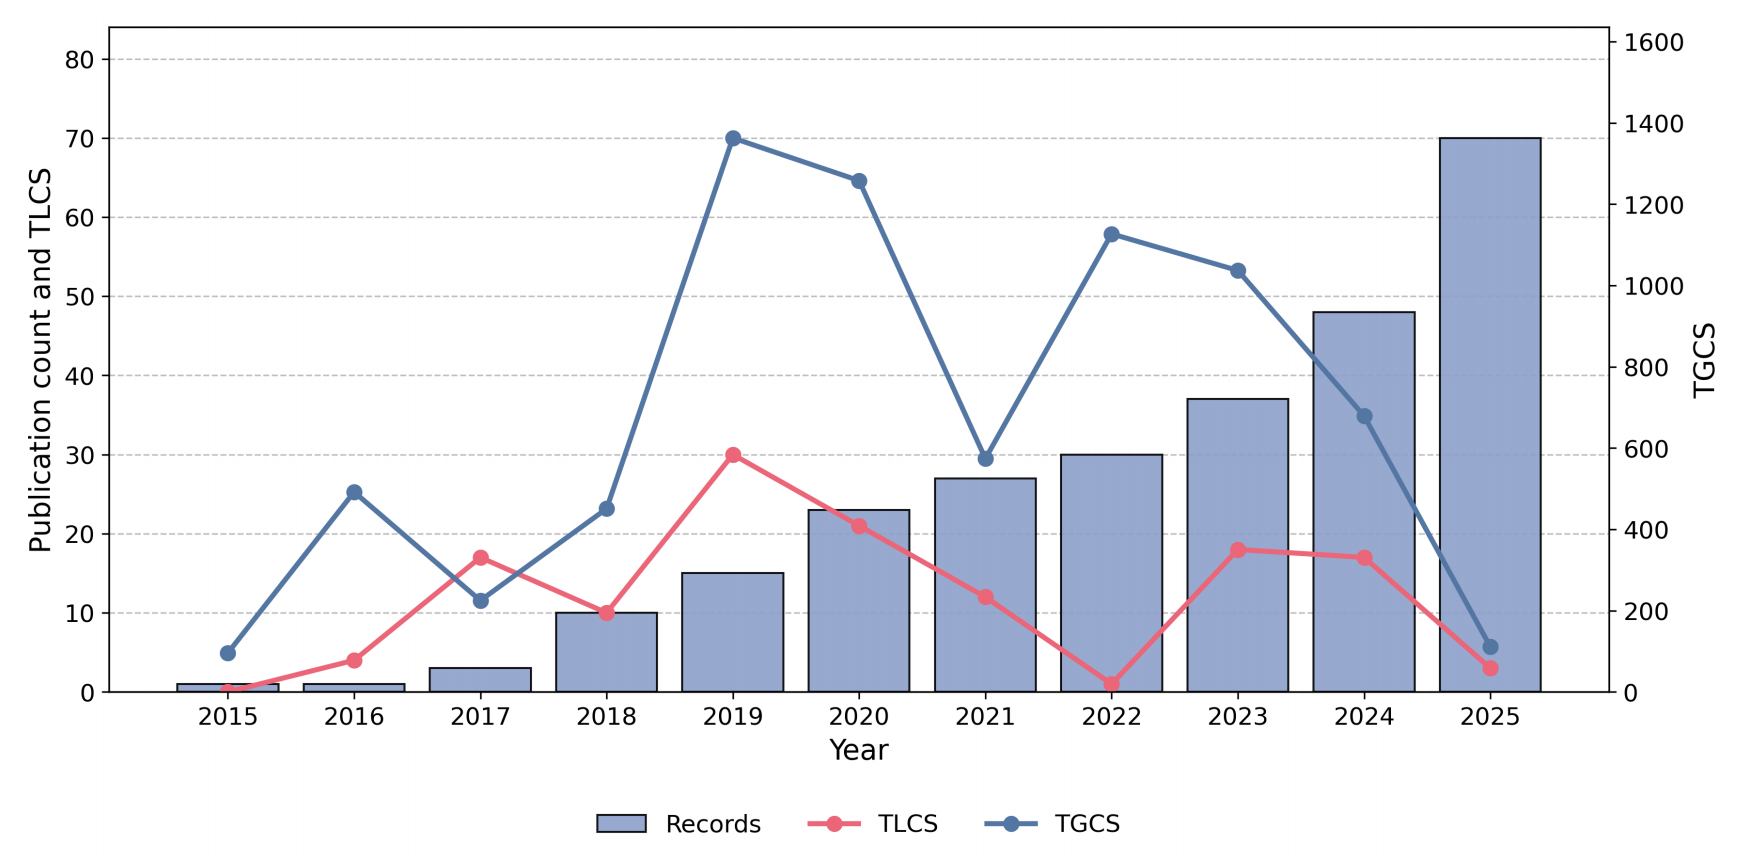
\includegraphics[width=0.75\columnwidth]{picture_2.png}
	\caption{Yearly publication output, TLCS, and TGCS of LULC research (2016--2025).}
	\label{fig:pub_trends}
\end{figure}

The period 2006--2014 is not explicitly detailed in the figure due to the negligible number of publications; however, the single relevant paper published in 2015 is included to mark the onset of research growth. As shown in the figure, the annual volume of publications has exhibited a consistent upward trend. This growth is primarily attributed to the rapid advancement of deep learning algorithms and the continuous enhancement of computational power \citep{ORIGma2019deep}. Notably, the final three years (2023--2025) represent the peak of productivity, with 37, 48, and 70 papers published, respectively \citep{ORIGtuia2023toward}.

While publication volume is a reliable indicator of research activity, it does not fully capture academic influence. To address this, TLCS and TGCS based on citation counts are employed to gauge scholarly impact. Notably, TGCS values are generally significantly higher than TLCS, as they encompass citations from the entire Web of Science database rather than just within the selected local dataset \citep{ORIGbornmann2011citation}.

TLCS reached its peak in 2019 (30), indicating that papers published in this year have attracted substantial attention within the specialized LULC community. Analysis reveals that two highly cited papers were the primary contributors to this peak: ``Advanced Multi-Sensor Optical Remote Sensing for Urban Land Use and Land Cover Classification: Outcome of the 2018 IEEE GRSS Data Fusion Contest'' (TLCS=17) \citep{21} and ``Combining Sentinel-1 and Sentinel-2 Satellite Image Time Series for land cover mapping via a multi-source deep learning architecture'' (TLCS=8) \citep{22}. Furthermore, although 2017 had a lower volume of publications, it maintained a relatively high TLCS. This is largely due to the influential work ``Hyperspectral and LiDAR Data Fusion Using Extinction Profiles and Deep Convolutional Neural Network'' (TLCS=15) \citep{23}. Given that deep learning and multi-source fusion are contemporary research hotspots, these studies have naturally attracted extensive attention.

TGCS similarly peaked in 2019 (1363), driven by the aforementioned works and complemented by ``Urban Tree Species Classification Using a WorldView-2/3 and LiDAR Data Fusion Approach and Deep Learning'' \citep{ORIG26}. A secondary peak in TGCS occurred in 2020 (1258), aligning with the TLCS trend. In this year, ``Cloud removal in Sentinel-2 imagery using a deep residual neural network and SAR-optical data fusion'' \citep{27} contributed significantly with 345 global citations. Interestingly, despite a very low publication count in 2016, the year achieved a remarkably high TGCS due to the seminal work ``Deep Learning Earth Observation Classification Using ImageNet Pretrained Networks'' \citep{28}, which contributed 492 citations. 

It is obvious that high-impact studies consistently focus on the intersection of deep learning and multi-source fusion. We also observe local peaks in the 2023 TLCS and 2022 TGCS following minor declines, which may be attributed to the delayed citation window effect \citep{ORIG4,ORIGbornmann2011citation}. Conversely, the scores for 2024 and 2025 remain relatively low, as newly published papers typically require several years to accumulate significant citation counts.


\subsection{Core Journals, Authors, Institutions, and Countries}

\subsubsection{Active Journals}


Scientific journals serve as the primary conduits for disseminating research findings and academic activities. The 261 publications analyzed in this study were distributed across 81 different journals. The top ten journals ranked by publication count, Local Citation Score (TLCS), and Total Global Citation Score (TGCS) are summarized in Fig.~\ref{fig:journal_impact}.
\begin{figure}[htb!] 
	\centering
	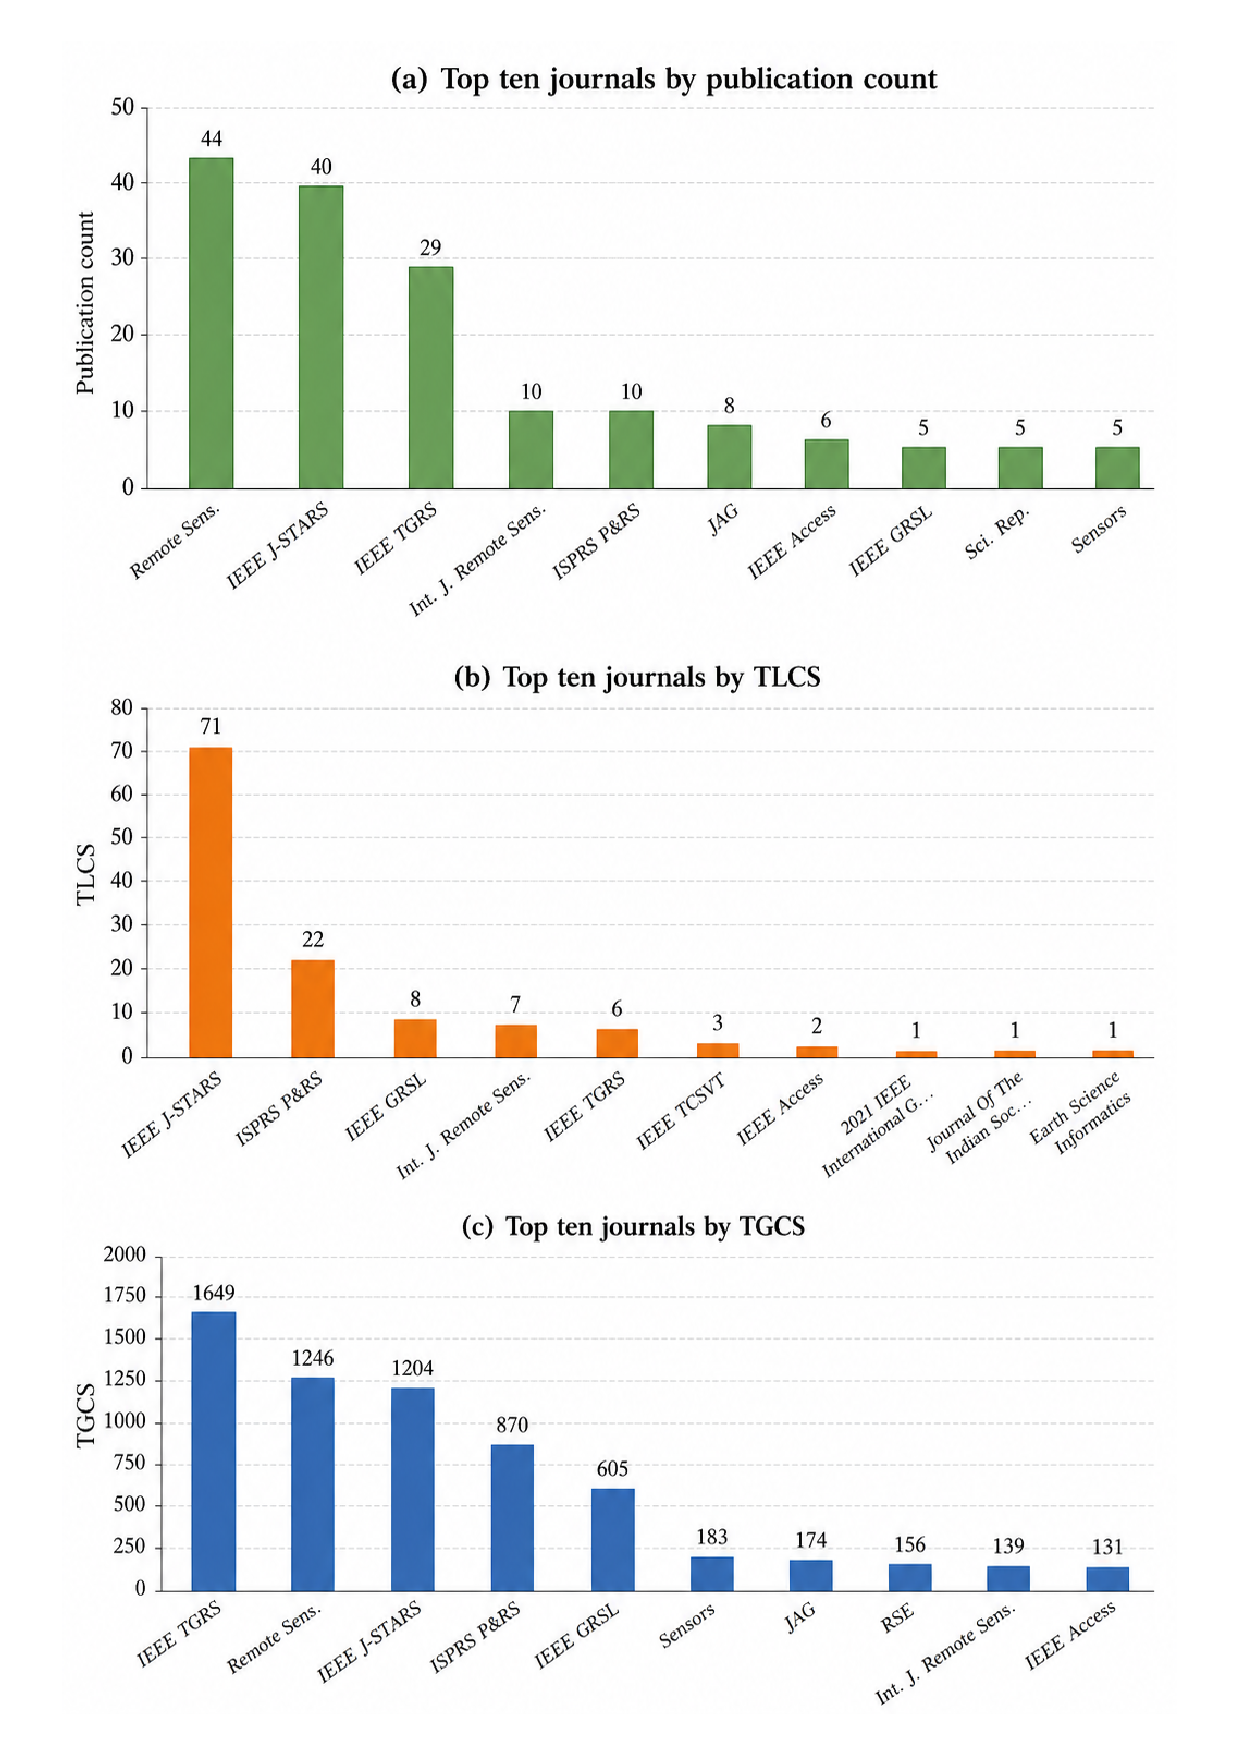
\includegraphics[width=0.75\columnwidth]{Figures/Picture_3.pdf} 
	\caption{Publication count, TLCS, and TGCS per journal (2006--2025).}
	\label{fig:journal_impact}
\end{figure}


According to Fig.~\ref{fig:journal_impact}(a), \textit{Remote Sensing} ranks first in terms of publication volume, making it the most active journal in the LULC research domain. However, its TLCS (7) only ranks fourth, showing a significant discrepancy compared to its high TGCS (1246). This may be attributed to its status as an open-access journal with a broad and multidisciplinary scope (covering ecology, agriculture, hydrology, etc.). Consequently, only a fraction of its total papers, those highly aligned with deep learning and remote sensing processing, are cited within this local sample set (low TLCS), whereas its wide global audience leads to high cross-disciplinary citations (high TGCS).

In contrast, \textit{IEEE J-STARS} ranks first in TLCS and third in TGCS (Fig.~\ref{fig:journal_impact}(b, c)), indicating that its publications are not only highly cited within the LULC community but also attract extensive attention from the broader scientific world. Furthermore, \textit{IEEE TGRS} leads in TGCS (1649), which is consistent with its reputation as one of the oldest and most prestigious top-tier journals in the remote sensing field since 1963.




\subsubsection{Important Authors}

Identifying key authors helps researchers grasp research hotspots and academic trends. In this study, 1,083 authors contributed to the 261 analyzed papers. The authors were ranked based on publication count, TLCS, and TGCS, as illustrated in Fig.~\ref{fig:author_impact}. 



\begin{figure}[htb!] 
	\centering
	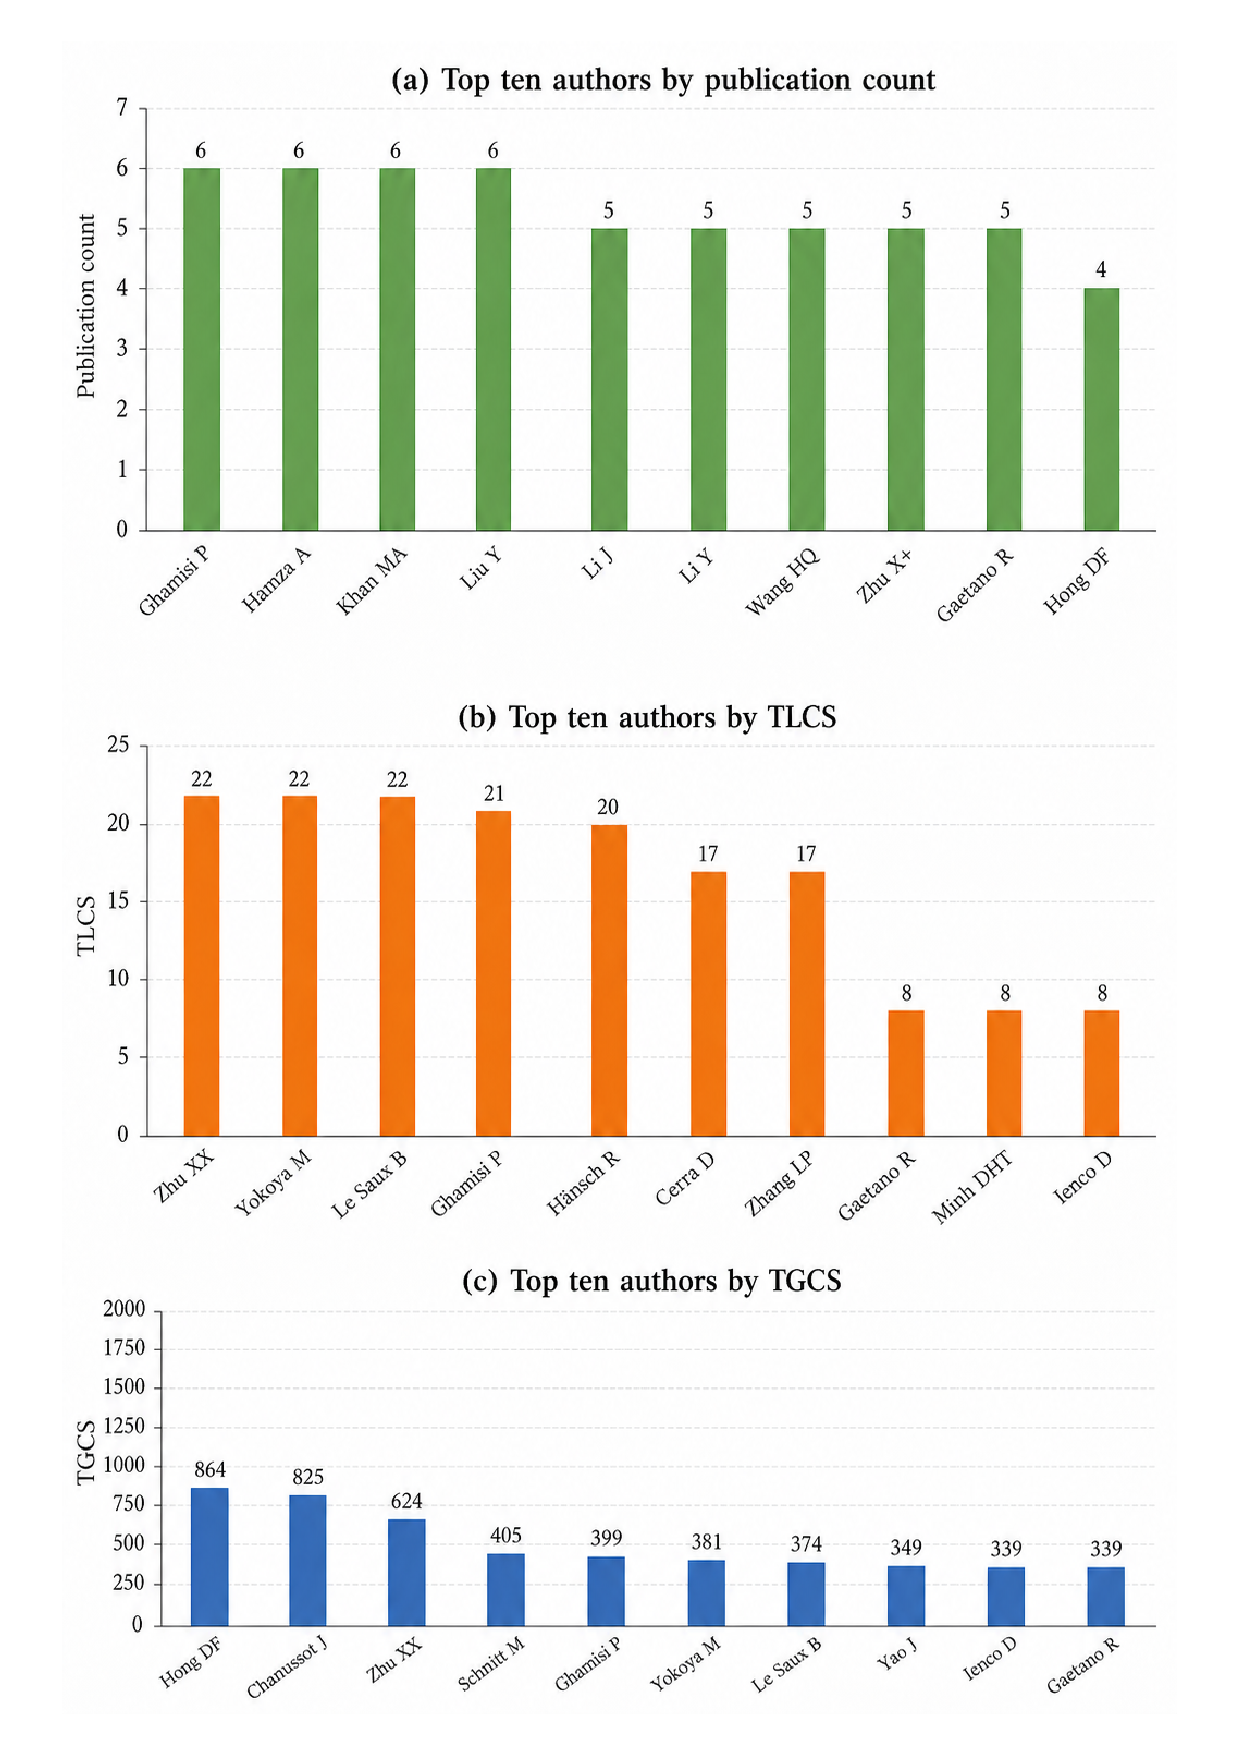
\includegraphics[width=0.75\columnwidth]{Figures/Picture_4.pdf} 
	\caption{Publication count, TLCS, and TGCS per author for LULC research (2006--2025).}
	\label{fig:author_impact}
\end{figure}

While Ghamisi P., Hamza A., Khan M. A., and Liu Y. lead in publication count with six papers each, further analysis of Fig.~\ref{fig:author_impact} (b, c) reveals that only Ghamisi P. maintains a top-ten ranking in both TLCS (5th, 21) and TGCS (5th, 399). This demonstrates his significant contribution to both the local community and global impact. Notably, Zhu X. X., Yokoya N., and Le Saux B. also exhibit high TLCS values (22 each). The collaborative work by Ghamisi P. and Zhu X. X., ``Hyperspectral and LiDAR Data Fusion Using Extinction Profiles and Deep Convolutional Neural Network'' \citep{23}, contributed a notable TLCS of 15. The frequent collaboration between these two authors and others highlights their roles as influential academic partners. From a global perspective, Hong D. F. shows the greatest influence in TGCS, primarily due to the work of 2022 ``Convolutional Neural Networks for Multimodal Remote Sensing Data Classification'' \citep{2}, which achieved a TGCS of 450.


\subsubsection{Active Institutions and Main Countries}
Institutions play a pivotal role in analyzing global developmental trends within a specific academic field. By calculating the affiliations of all authors, a total of 420 institutions were identified. The statistical results for publication volume, Local Citation Score (TLCS), and Total Global Citation Score (TGCS) for each institution are summarized in Fig.~\ref{fig:inst_impact}. Wuhan University leads with 24 publications, making it the most active institution in this field. The Chinese Academy of Sciences (CAS) and Huazhong University of Science and Technology follow in second and third place, with 22 and 10 publications, respectively. Notably, the output from Wuhan University and CAS significantly exceeds that of other institutions.



In terms of TLCS rankings, the German Aerospace Center (DLR) and Zhuhai University hold prominent positions. Wuhan University, PIEAS, and University of Technology Sydney follow closely, each with a TLCS of 22. These results indicate that Wuhan University not only maintains high annual output but also commands significant academic recognition within the field. Regarding TGCS (as shown in Fig.~\ref{fig:inst_impact}(c)), CAS and Zhejiang University emerge as the leading global institutions. 


National contribution is another critical dimension for assessing academic activity in LULC. The retrieved literature spans 134 countries, demonstrating the worldwide importance of this field. The top ten countries by publication volume account for 89.30\% of the total output. Fig.~\ref{fig:country_impact} illustrates the distribution of the top ten countries across the three metrics: publication count, TLCS, and TGCS. Germany and China rank within the top three across all three metrics. However, raw publication counts do not fully reflect national research intensity; contributions are better assessed relative to population size and the number of active PhD researchers in each country. When these normalization factors are considered, the relative standing of some countries may shift. Furthermore, several prestigious institutions are based in these two nations, underscoring their dominant influence in both the local academic community and the global scientific sphere. Six countries, including China, Germany, India, France, the UK, and Japan, consistently rank among the top ten across all indicators. 



As shown in Figs.~\ref{fig:country_impact} and~\ref{fig:country_collab_compact}, China holds an absolute leading position, with its total publication volume far exceeding that of other nations. The vast majority of China's research is conducted independently within the country (indicated by the large light-green portion in Fig.~\ref{fig:country_collab_compact}), while multi-country collaborative papers represent a smaller fraction. This spatial distribution is further elucidated in Fig.~\ref{fig:collab_map}, which visualizes the intensity and geographical direction of these partnerships. Despite the high proportion of independent research, China maintains a robust international network, with significant collaborative links extending primarily to North America, Europe, and Australia.

Other countries exhibit distinct collaboration patterns: India and Germany also show a high proportion of independent research. In contrast, while the total publication volumes for the USA, South Korea, Iran, and Australia decrease sequentially, their proportion of international collaborative papers (indicated in red in Fig.~\ref{fig:country_collab_compact}) is significantly more prominent. As illustrated in the geographical distribution (Fig.~\ref{fig:collab_map}), these nations act as key nodes in the global LULC research network, facilitating transcontinental knowledge flow. This reflects that while China leads in volume through primarily independent research, followed by India and Germany, other nations leverage international cooperation more extensively to enhance their scientific impact and resource sharing.

\begin{figure}[htb!] % [p] 标签确保图片独占一页，符合学术排版规范
	\centering
	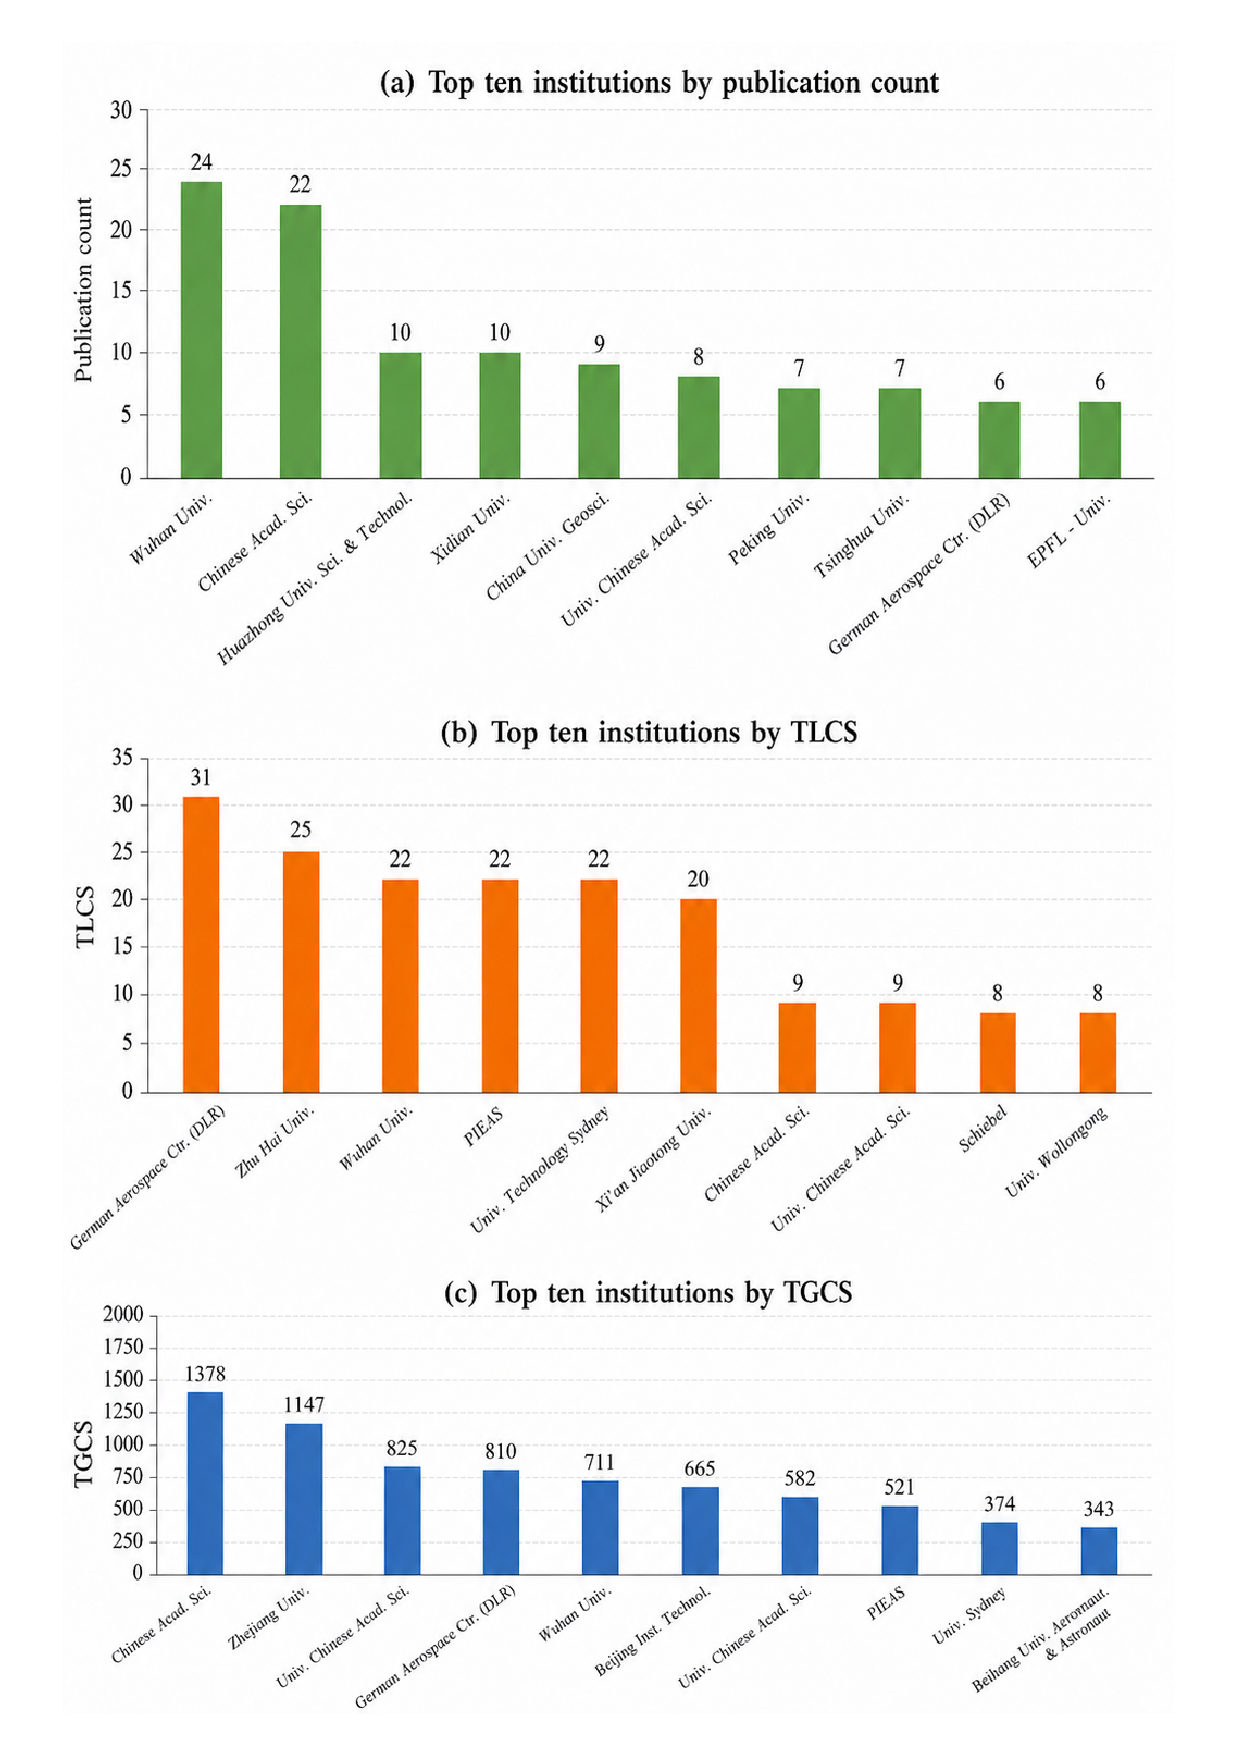
\includegraphics[width=0.75\columnwidth]{Figures/Picture_5.pdf} 
	\caption{Publication volume, TLCS, and TGCS per institution for LULC research (2006--2025).}
	\label{fig:inst_impact}
\end{figure}


\begin{figure}[htb!] % [p] 标签确保图片独占一页，符合学术排版规范
	\centering
	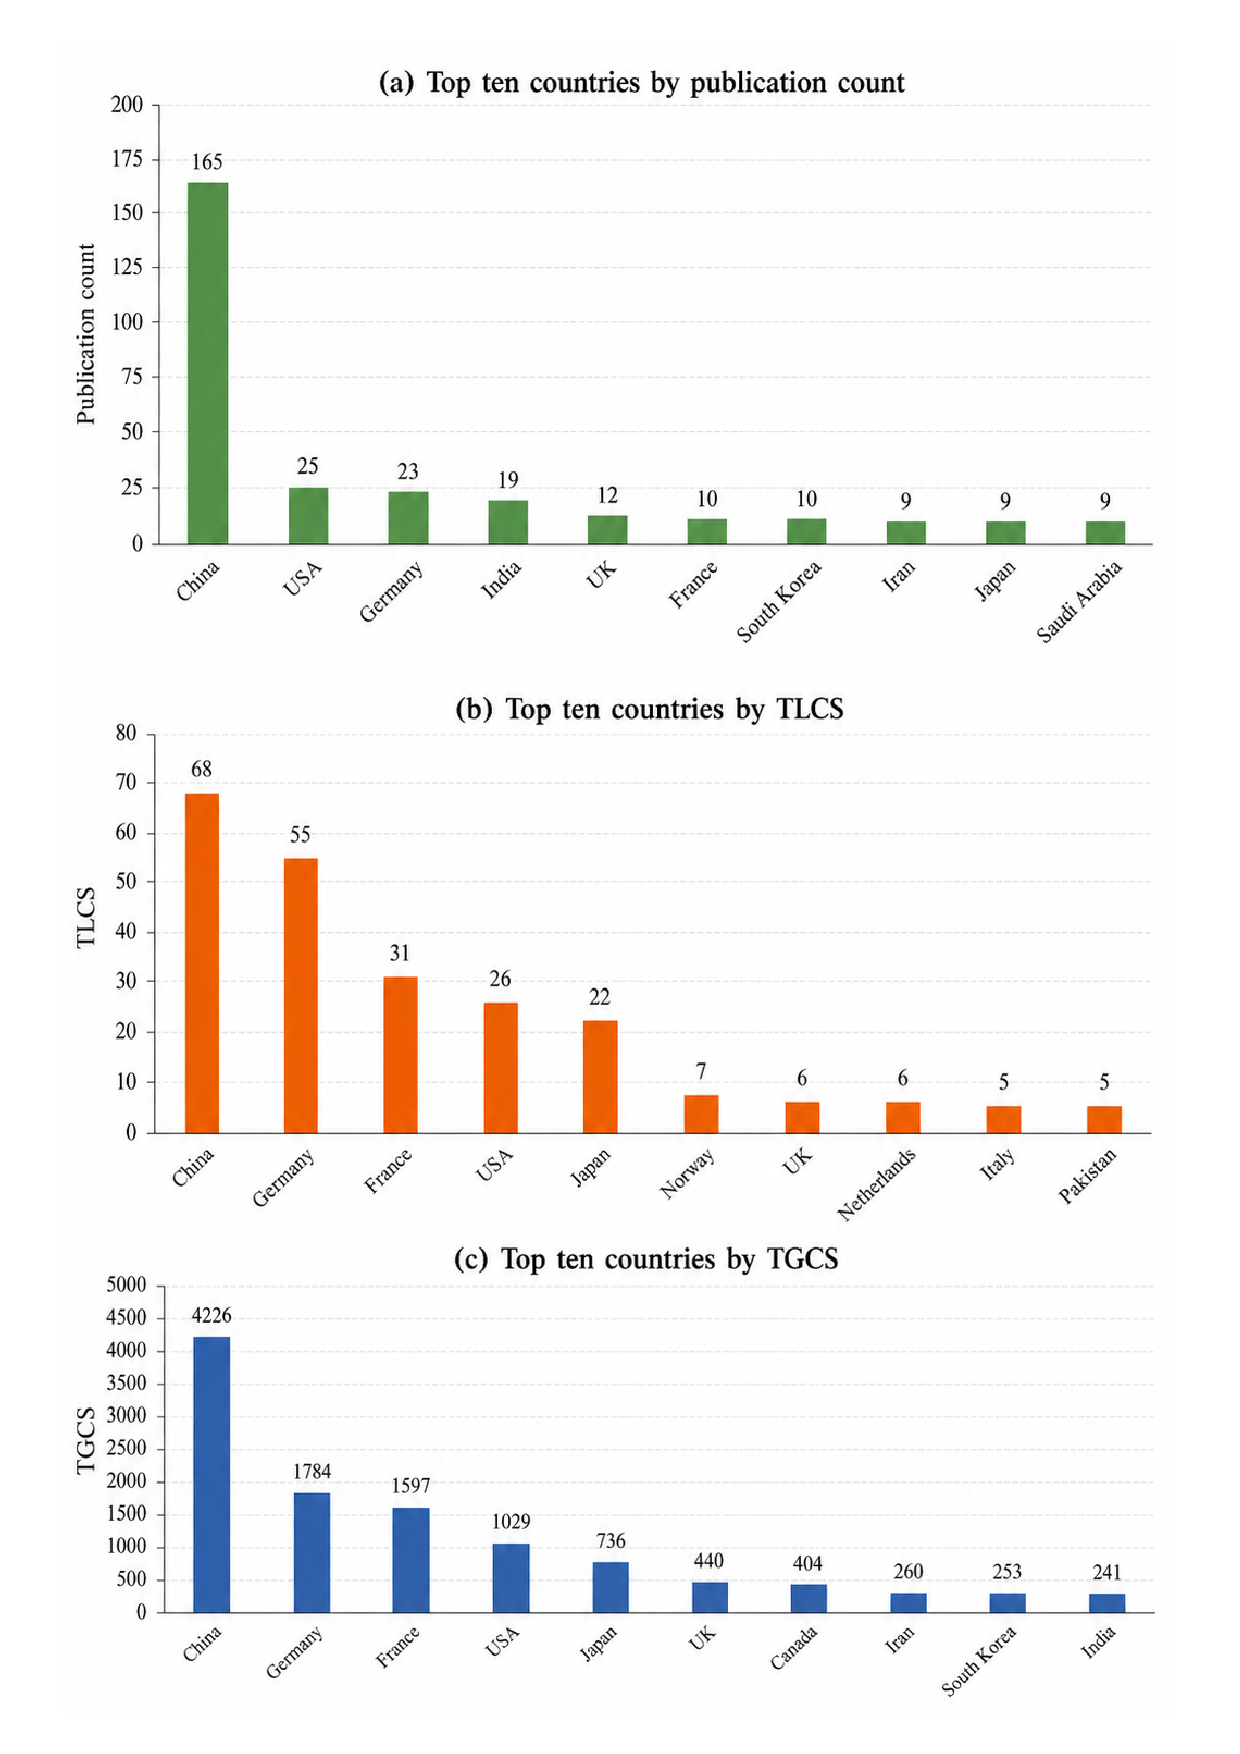
\includegraphics[width=0.75\columnwidth]{Figures/Picture_6.pdf} 
	%    \vspace{-10pt} 
	\caption{Top ten countries ranked by publication volume, TLCS, and TGCS for LULC research (2006--2025).}
	\label{fig:country_impact}
\end{figure}

% --- 修改后的图 7 和 图 8 布局 ---
\begin{figure}[htb!] % [p] 标签确保图片独占一页，符合学术排版规范
	\centering	
	% 图 7
	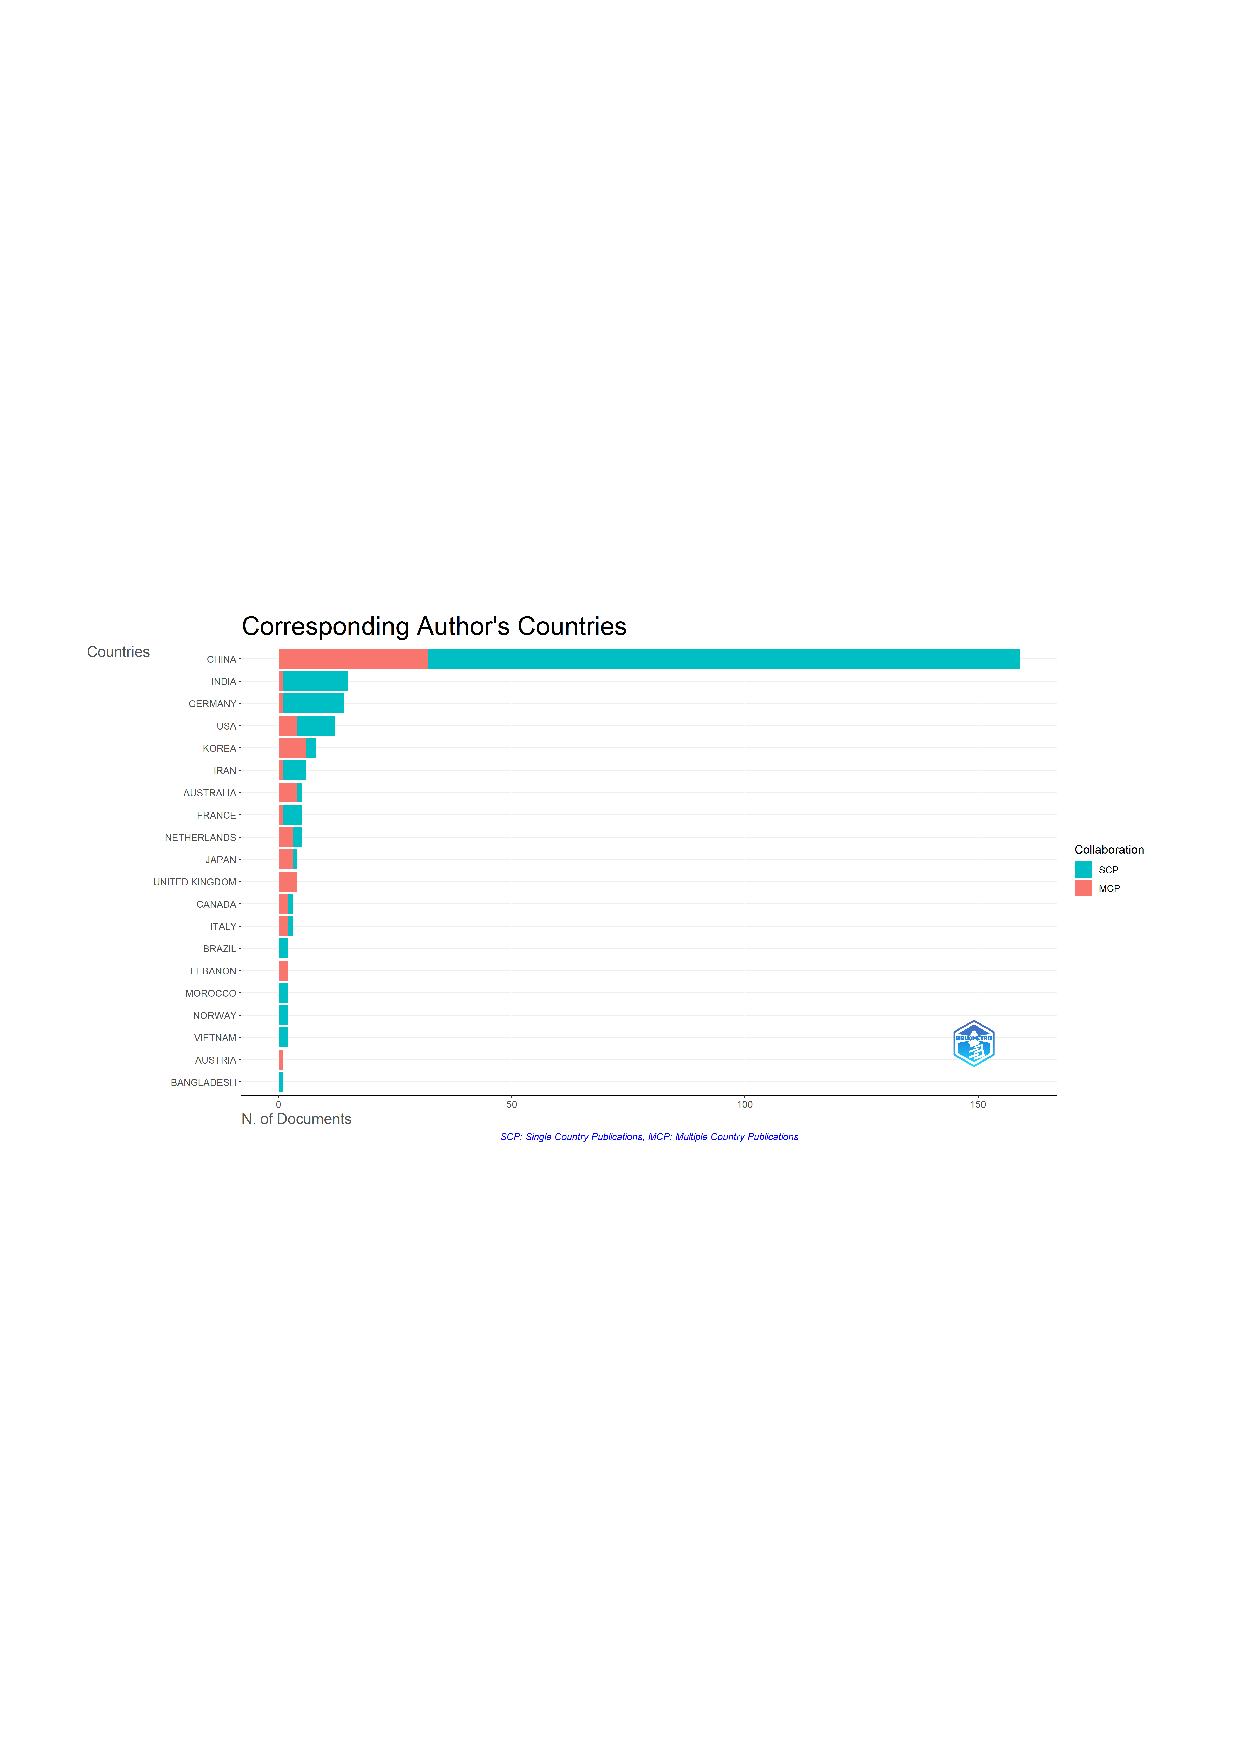
\includegraphics[width=1.0\textwidth, height=0.38\textheight, keepaspectratio]{Figures/picture_7.pdf}
	\vspace{-10pt}
	\caption{Collaboration analysis of major countries: MCP versus SCP. Here, MCP denotes Multiple Country Publication (i.e., co-authors from two or more different countries), while SCP denotes Single Country Publication (i.e., all authors affiliated with the same country)}
	\label{fig:country_collab_compact}
	\vspace{10pt} % 两图间距
	
	% 图 8
	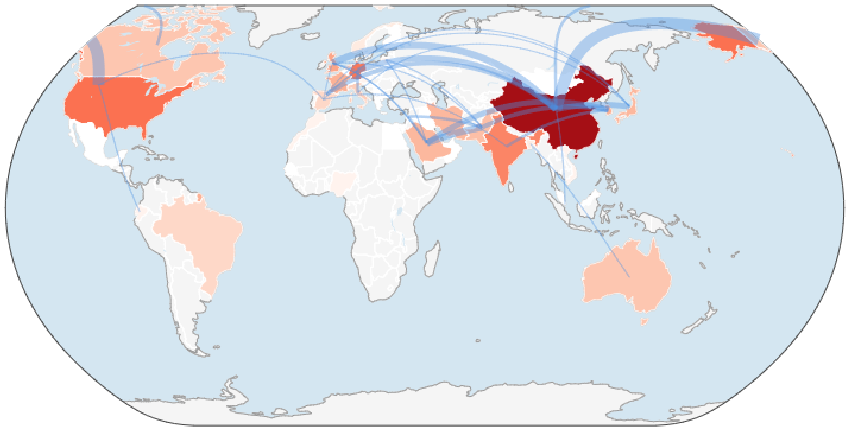
\includegraphics[width=1.0\textwidth, height=0.38\textheight, keepaspectratio]{Figures/newplot.pdf}
	\vspace{-10pt}
	\caption{Geographical distribution of international research collaborations.}
	\label{fig:collab_map}
\end{figure}

\section{Results and Discussion}

\subsection{Keyword Co-occurrence and Temporal Evolution}

In this study, VOSviewer software was employed to conduct a keyword hotspot analysis on 261 publications related to LULC simulation indexed in the Web of Science database from 2006 to 2025. The analysis reveals the core research trends and the evolutionary path of the field, as illustrated in Fig.~\ref{fig:keyword_evolution}. Notably, due to the limited number of publications between 2006 and 2015, keyword visualization for that specific decade is omitted.

\begin{figure*}[t]
	\centering
	% --- 第一张图 (原 Figure 9) ---
	\makebox[\textwidth][c]{
		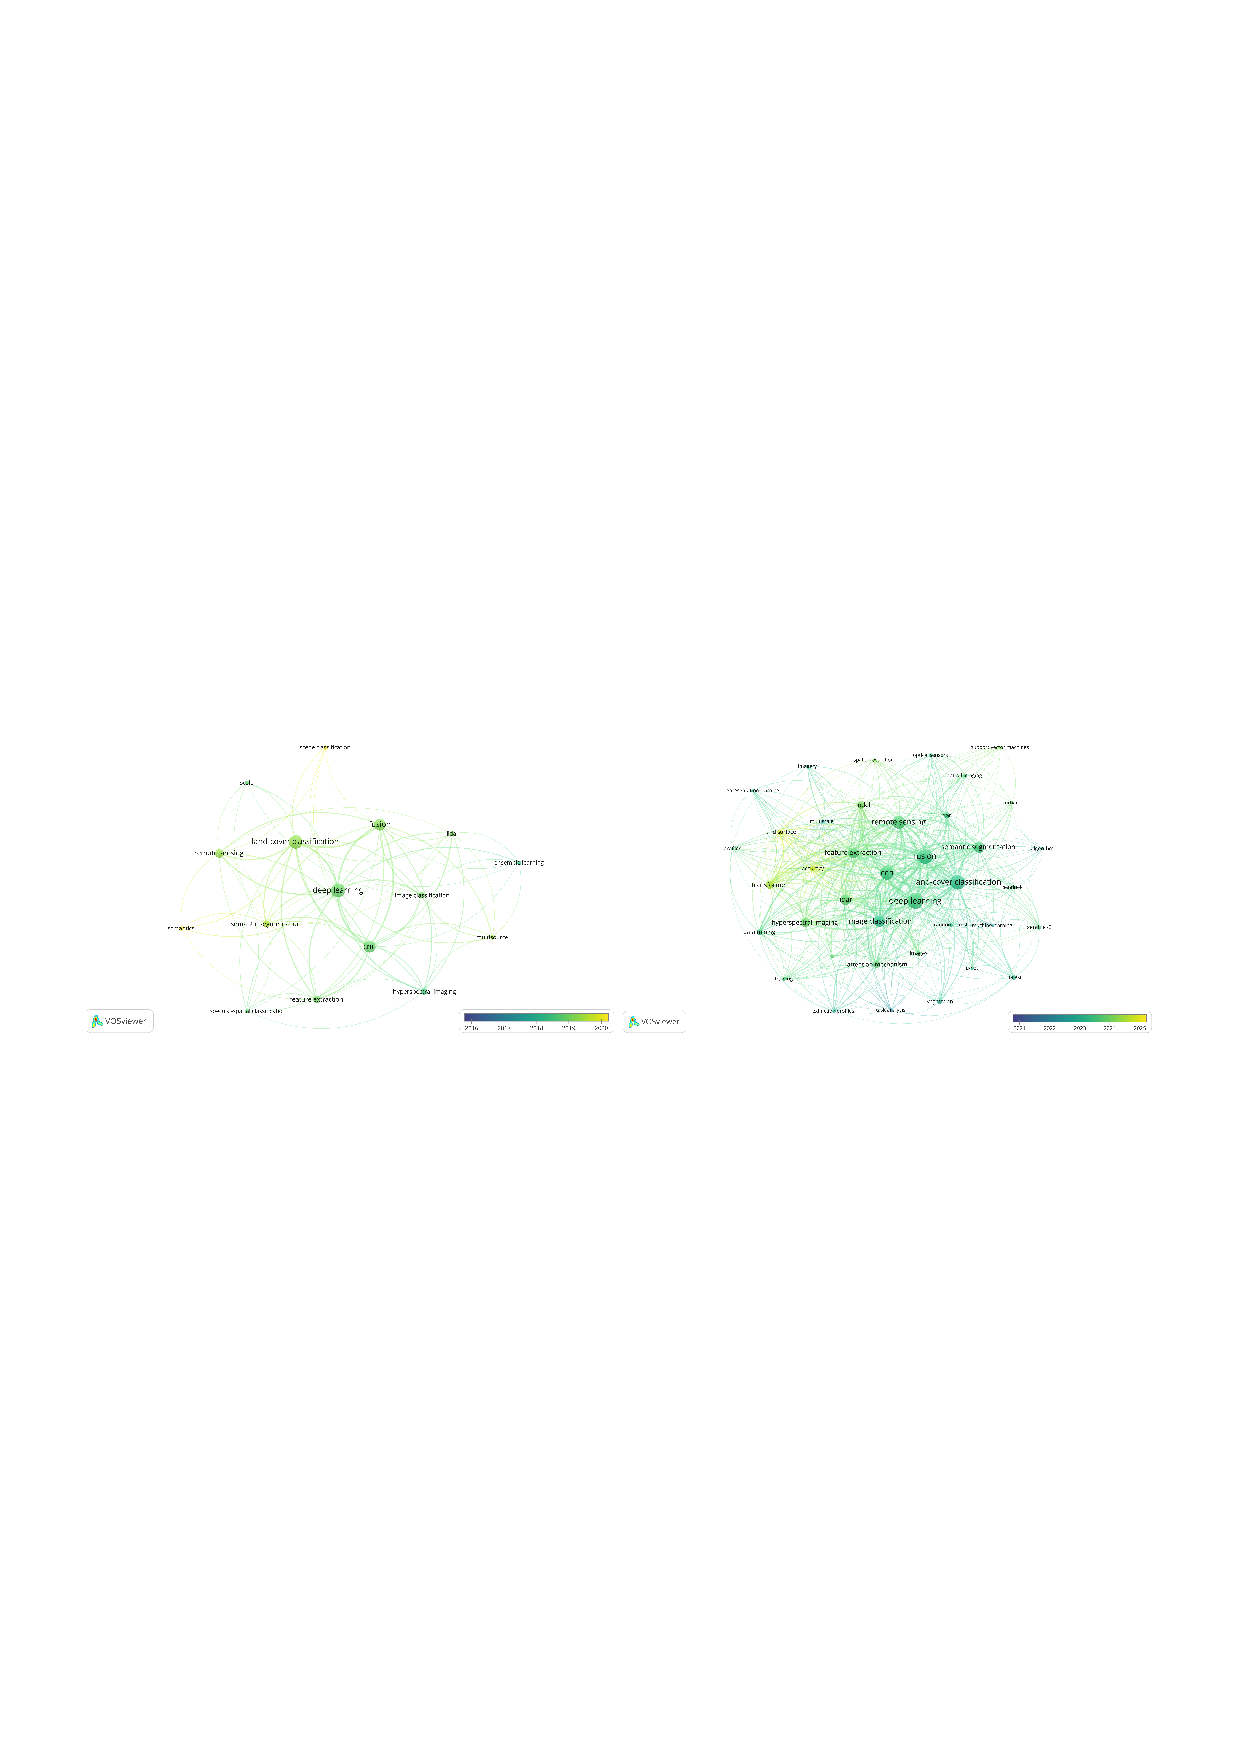
\includegraphics[width=1.05\textwidth]{Figures/picture_8.pdf}}
	%    \vspace{-5pt} 
	\caption{Keyword co-occurrence network and temporal evolution in LULC simulation research (2016--2025): (left) 2016--2020 period; (right) 2021--2025 period.}
	\label{fig:keyword_evolution}
	
	\vspace{20pt} % 在两张图之间增加明显的间距
	
	% --- 第二张图 (原 Figure 10) ---
	\includegraphics[width=0.85\textwidth]{Figures/new_all.pdf}
	%    \vspace{-5pt}
	\caption{Comprehensive keyword co-occurrence network of LULC simulation research (2006--2025), highlighting the integration of deep learning and multi-source data fusion.}
	\label{fig:keyword_all}
\end{figure*}

As shown in Fig.~\ref{fig:keyword_evolution}, during the 2016--2020 period (left portion of the network), the focus of LULC simulation research was concentrated on keywords such as ``land-classification'', ``deep learning'', ``fusion'', and ``CNN''. These keywords recorded occurrences of 33, 30, 23, and 23, respectively, with their Total Link Strength (TLS) ranking highest at 101, 84, 72, and 72. This indicates that the academic community during this stage began to extensively integrate multi-source data fusion with deep learning architectures \citep{23}, witnessing the evolution of LULC research into a multi-disciplinary intersection \citep{ORIG6}.

According to the analysis of the 2021--2025 period (right portion of Fig.~\ref{fig:keyword_evolution}), research hotspots have further intensified around four distinct clusters. The occurrences for ``deep learning'', ``fusion'', and ``CNN'' soared to 104, 94, and 83, with their TLS reaching 422, 422, and 399, respectively. The ``remote sensing'' node also appears prominently with 69 occurrences and a TLS of 351, serving as the core infrastructural support upon which all thematic research is built. Similarly, the ``land-cover classification'' node remains highly conspicuous, confirming its status as a classic and continuously trending task in the remote sensing domain \citep{cao2020urban}.

% --- 针对新图片 Figure 10 扩充的分析内容 ---
To gain a more holistic perspective, Fig.~\ref{fig:keyword_all} presents the comprehensive keyword co-occurrence network across the entire study period. The dense interconnection between ``deep learning'' and various sensor-specific nodes, such as ``hyperspectral imaging'', ``LiDAR'', and ``SAR'' underscores a paradigm shift toward high-dimensional data processing. Notably, emerging keywords like ``Transformer'', ``attention mechanism'', and ``Mamba'' occupy strategic positions within the network. This suggests a transition from local feature extraction to global contextual modeling in LULC simulation tasks.

In contrast, nodes representing traditional methods, such as ``support vector machines,'' ``optical sensors,'' and ``random forest'' \citep{belgiu2016random} are smaller and characterized by greener hues in the temporal overlay. This suggests that while they remain essential baseline or complementary techniques, their relative research heat has declined compared to modern deep learning approaches. Meanwhile, nodes related to multi-source data fusion maintain a significant scale. This demonstrates that multi-source remote sensing data fusion remains a consistent research priority, increasingly coupled with deep learning in recent years. Furthermore, the appearance of ``representation learning'' and ``self-attention'' on the periphery of the network marks the latest frontiers in the transition toward advanced feature extraction and autonomous model adaptation.

\subsection{Intellectual Structure}
To reveal the theoretical foundations and intellectual origins of this field, a document co-citation network was constructed using VOSviewer, as illustrated in Fig.~\ref{fig:intellectual_structure}. Co-citation analysis identifies the semantic relationships between documents based on their simultaneous citation patterns. The results reveal four distinct clusters, representing the knowledge lineage of deep learning-based LULC research \citep{19}:

% --- Figure 9: 知识基础结构图 (针对物理裁剪优化版) ---
\begin{figure}[!ht]
	\centering
	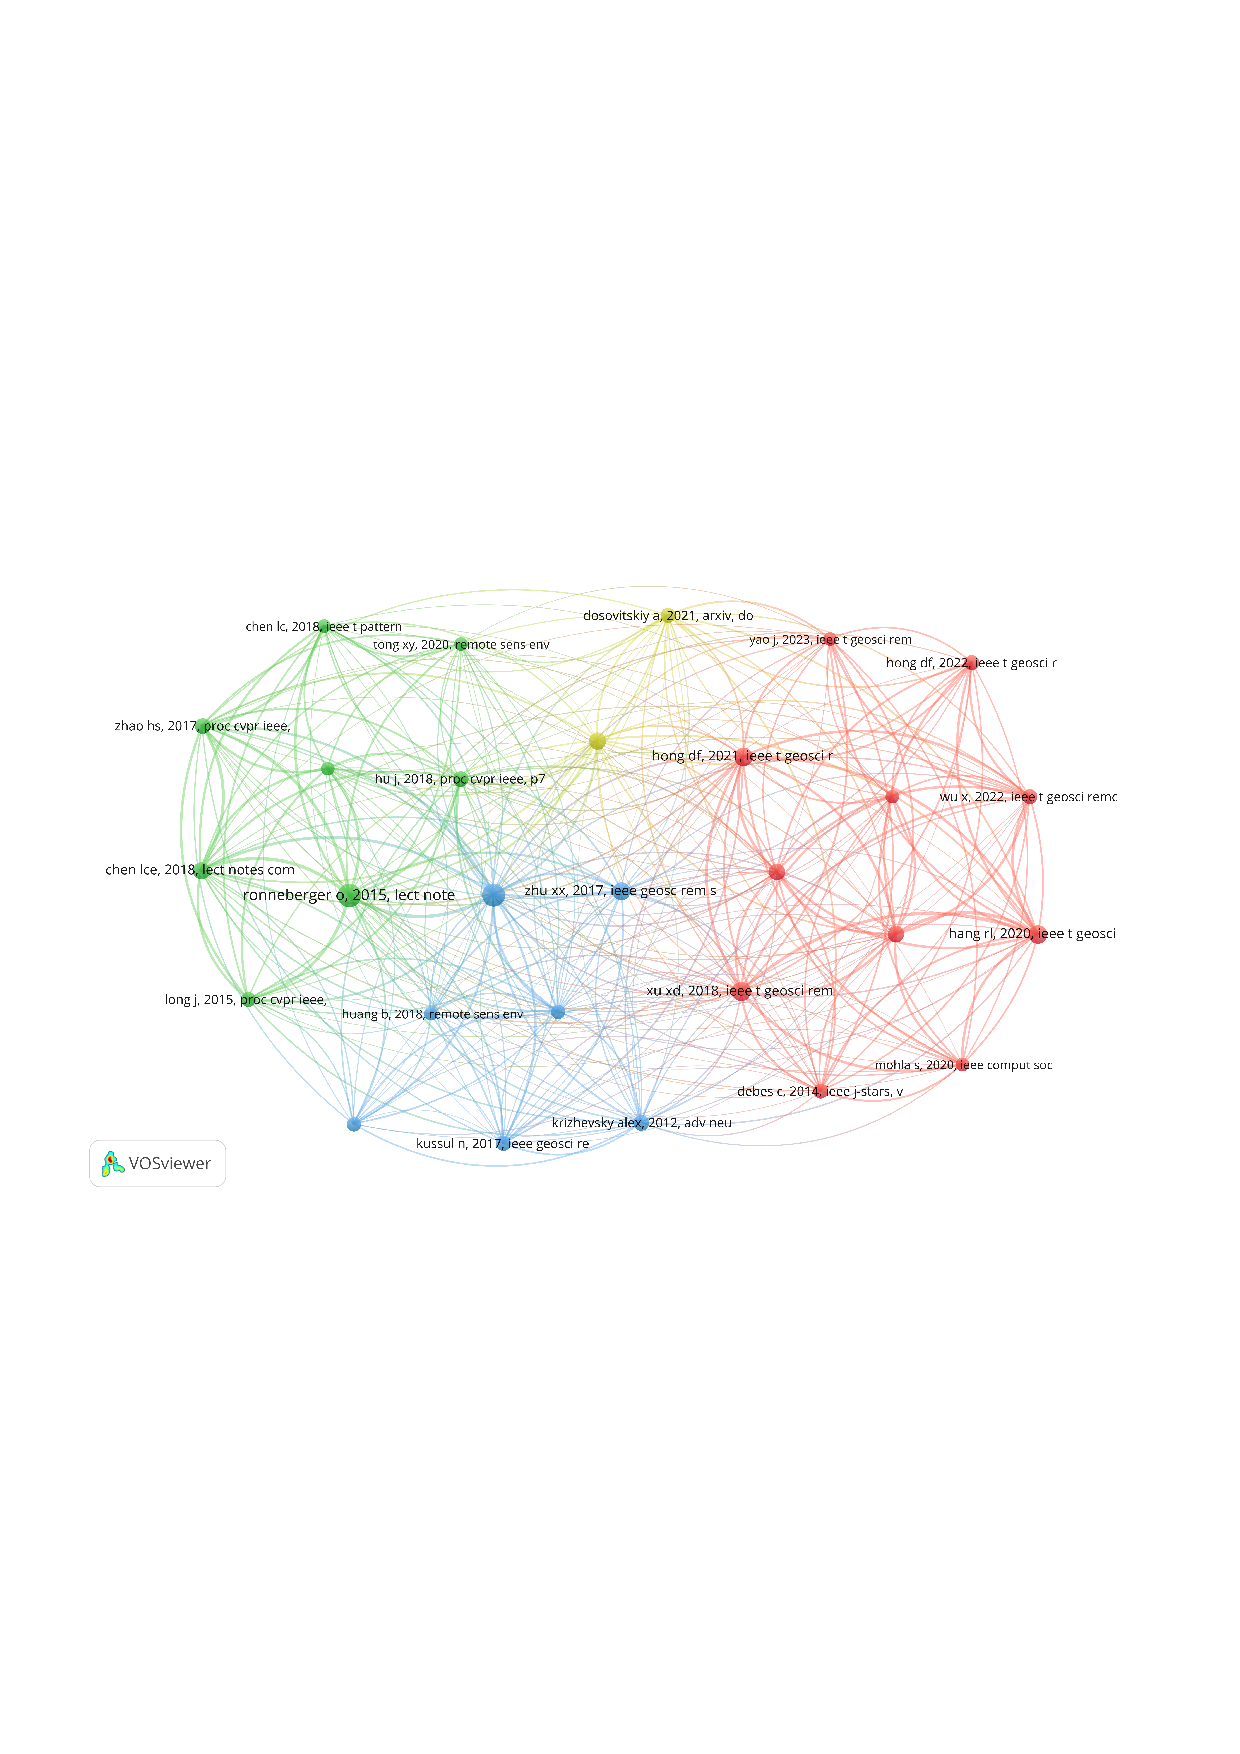
\includegraphics[width=1.0\columnwidth]{Figures/picture_9.pdf}
	\caption{Document co-citation network revealing the intellectual structure of LULC research.}
	\label{fig:intellectual_structure}
\end{figure}

\begin{enumerate}
	\item \textbf{Deep Learning Fundamentals (Blue Cluster):} This cluster represents the cornerstone of computer vision algorithms. Core nodes include Krizhevsky et al. (2012, AlexNet) and Simonyan et al. (2015, VGG) \citep{31,32}. These landmark studies introduced the AlexNet architecture and VGG network, respectively. Although originating from general computer vision, they provided the foundational CNN architectures that serve as primary feature extractors for remote sensing imagery. The highly cited work by Marmanis et al. (2016) directly bridges this cluster with remote sensing, marking the successful transfer of ImageNet pre-trained models to Earth observation tasks.
	
	\item \textbf{Semantic Segmentation Paradigm (Green Cluster):} This cluster focuses on ``pixel-to-pixel'' classification methods, which are critical for LULC mapping. Key nodes include Long et al. (2015, FCN) \citep{ORIG33} and Ronneberger et al. (2015, U-Net) \citep{34}. These studies established the ``encoder-decoder'' architecture, enabling end-to-end dense prediction. In the context of LULC, this paradigm shifted the research focus from patch-based classification to precise boundary delineation.
	
	\item \textbf{Multi-source Data Fusion (Red Cluster):} Dominated by scholars such as Ghamisi P., Zhu X.X., and Hong D.F., this cluster represents the specific application of deep learning to heterogeneous remote sensing data. This lineage originates from classical statistical modeling of sensor physics  and the establishment of rigorous evaluation frameworks for pixel-level fusion \citep{ORIG58}. Unlike the general-algorithm clusters, this group specifically addresses fusion challenges involving Hyperspectral (HSI), LiDAR, and SAR data. The dense connections within this cluster highlight the intensive academic efforts in developing specialized fusion modules to handle the unique physical attributes of remote sensing data.
	
	\item \textbf{Emerging Transformer Frontier (Yellow Cluster):} Representing the latest paradigm shift, this cluster centers on Dosovitskiy et al. (2021, Vision Transformer) \citep{35}. It marks the transition from local convolutional operations to global attention mechanisms. The emergence of this cluster echoes recent high-impact papers such as Yao et al. (2023, ExViT), indicating that the field is actively moving toward an era of foundation models capable of long-range spatial modeling of complex earth surfaces \citep{36}.
\end{enumerate}

%\FloatBarrier
\subsection{Analysis of Emerging Research Methods}
Prior to the dominance of deep learning, LULC research primarily relied on traditional machine learning algorithms and object-based analysis. As summarized in Table~\ref{tab:traditional_methods}, SVM and RF have long been considered benchmark methods due to their robustness with small samples and high-dimensional data.

\begin{table}[!ht]
	\centering
	\setlength{\belowcaptionskip}{5pt} 
	\caption{Traditional methods in LULC research.} 
	\label{tab:traditional_methods}
	\small 
	\renewcommand{\arraystretch}{1.4} 
	\begin{tabular}{@{} p{2.5cm} p{5.5cm} p{6.5cm} @{}} 
		\toprule
		\textbf{Method} & \textbf{Advantages} & \textbf{LULC Application Scenarios} \\ 
		\midrule
		SVM & Strong generalization with small samples. & Fine-classification with hyperspectral data. \\ \addlinespace[3pt]
		RF  & High accuracy and stability; resists overfitting. & Large-scale mapping on cloud platforms like GEE. \\ \addlinespace[3pt]
		ANN & Handles non-linear relationships effectively. & VHR imagery to reduce pixel fragmentation. \\ 
		\bottomrule
	\end{tabular}
\end{table}

% --- 衔接与分析段落 1：方法论分布 ---
To further quantify the shift toward modern architectures, we analyzed the distribution of methodological approaches within the sampled literature. Here, feature-level fusion has emerged as the absolute dominant paradigm, accounting for 80.9\% of the studies. This is followed by hybrid Data+Feature fusion (7.4\%) and decision-level fusion (4.3\%). This distribution underlines a significant shift in the research community towards integrating high-level semantic features rather than relying on raw signal concatenation.


% --- 衔接与分析段落 2：从方法论到核心技术热点 (Fig. 13) ---
The prevalence of feature-level fusion is deeply rooted in the surge of deep learning techniques. As shown in the keyword density visualization (Fig.~\ref{fig:keyword_density}), the absolute ``gravitational centers'' of the field are concentrated around ``deep learning'', ``fusion'', and ``CNN''. These nodes form the core technological drivers, where multi-scale feature extraction through CNN has become the standard implementation for achieving the high-level semantic integration mentioned. Notably, while traditional methods like SVM appear as lower-density peripheral nodes, the intense yellow clusters signify that the field has fully entered an era dominated by neural-based feature fusion.

\begin{figure}[htb!]
	\centering
	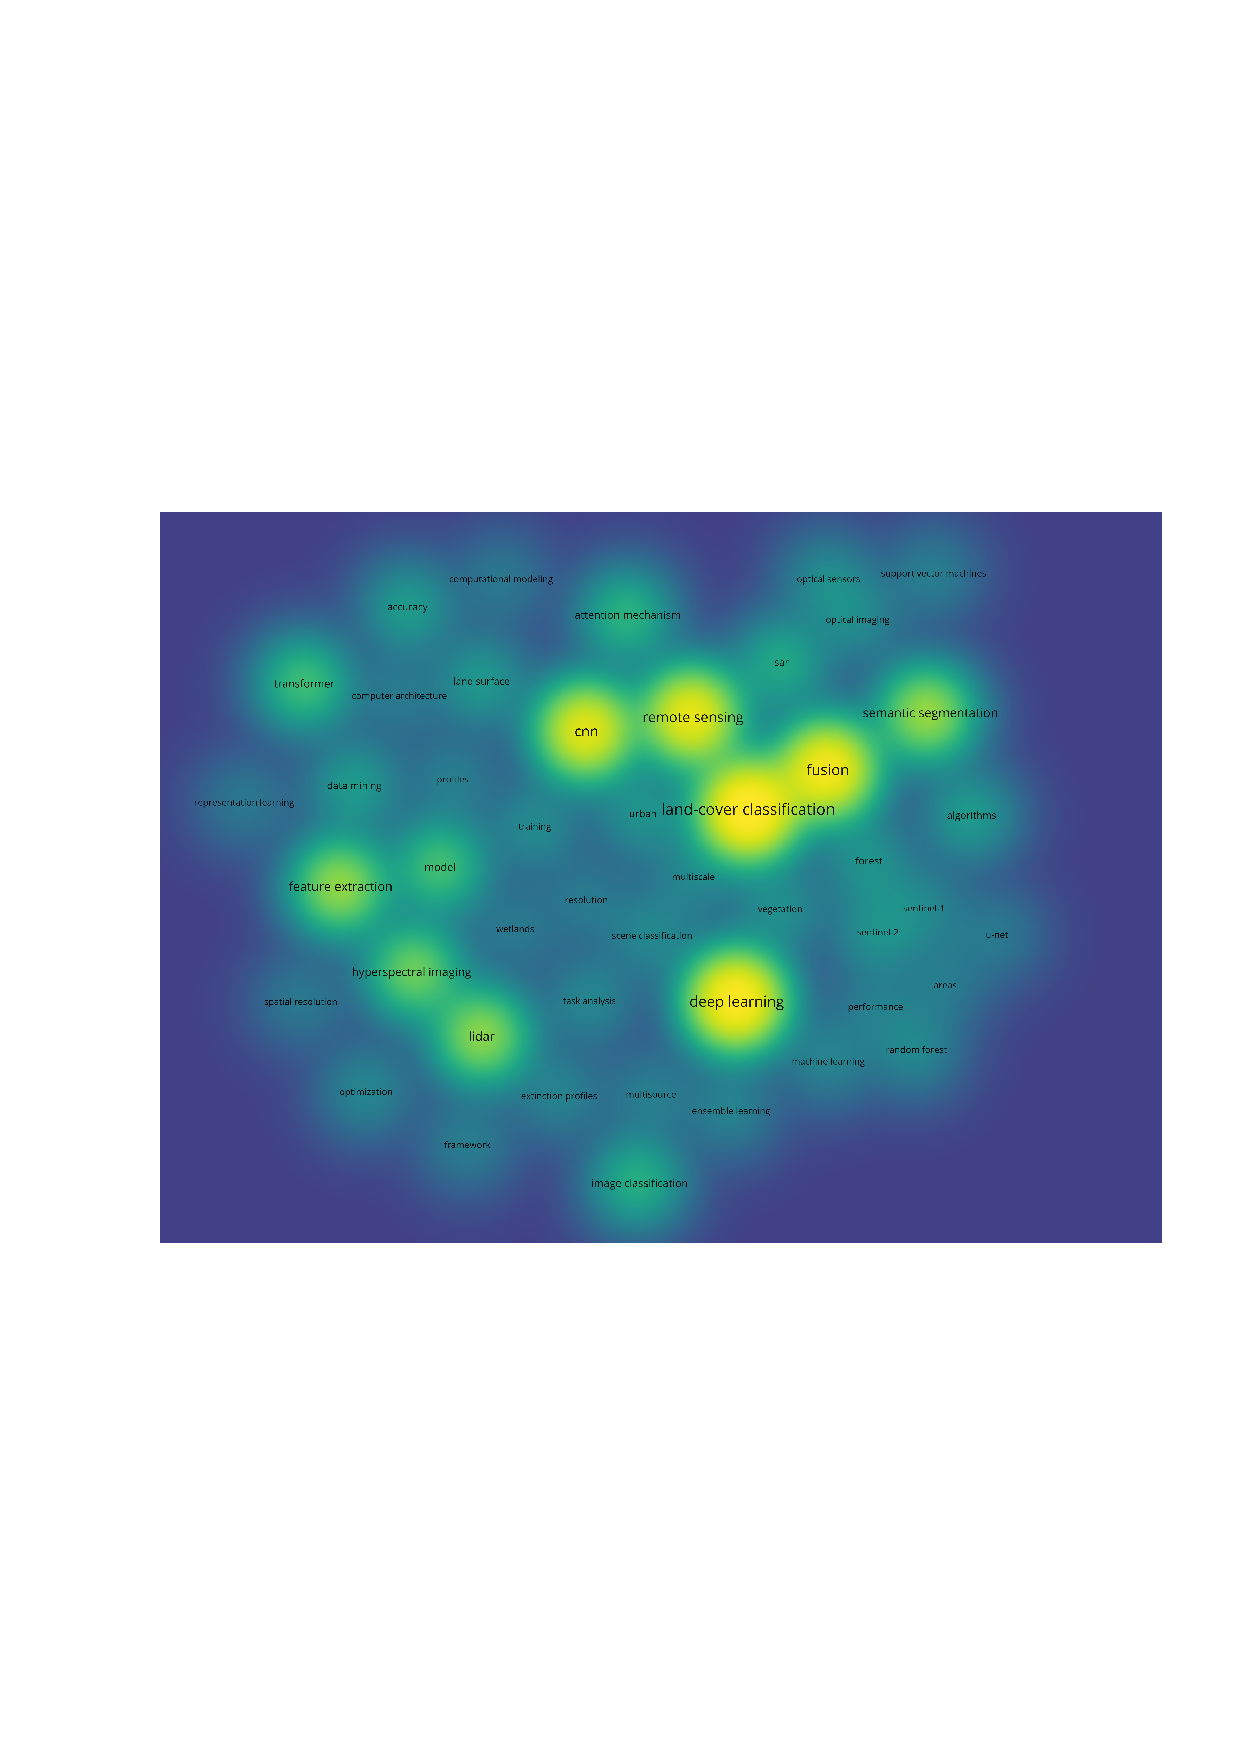
\includegraphics[width=0.85\columnwidth]{Figures/new_Relitu.pdf}
	\caption{Density visualization of keyword hotspots, identifying the core technological drivers within the LULC simulation domain.}
	\label{fig:keyword_density}
\end{figure}

% --- 衔接与分析段落 3：从技术热点到数据验证 ---
Currently, the maturation of these deep learning fusion models is heavily based on robust validation through benchmark datasets. The high-density focus on ``hyperspectral imaging'' and ``LiDAR'' in Fig.~\ref{fig:keyword_density} is directly reflected in the dataset utilization rankings. Our analysis (Fig.~\ref{fig:datasets_ranking}) reveals that Houston (25 studies) and Trento (15 studies) remain the most prevalent benchmarks. This concentration highlights the community's reliance on standardized, multi-modal data to evaluate the performance of feature-fusion architectures in complex urban and agricultural environments.

% --- Figure 14: 数据集排名柱状图 ---
\begin{figure}[!ht]
	\centering
	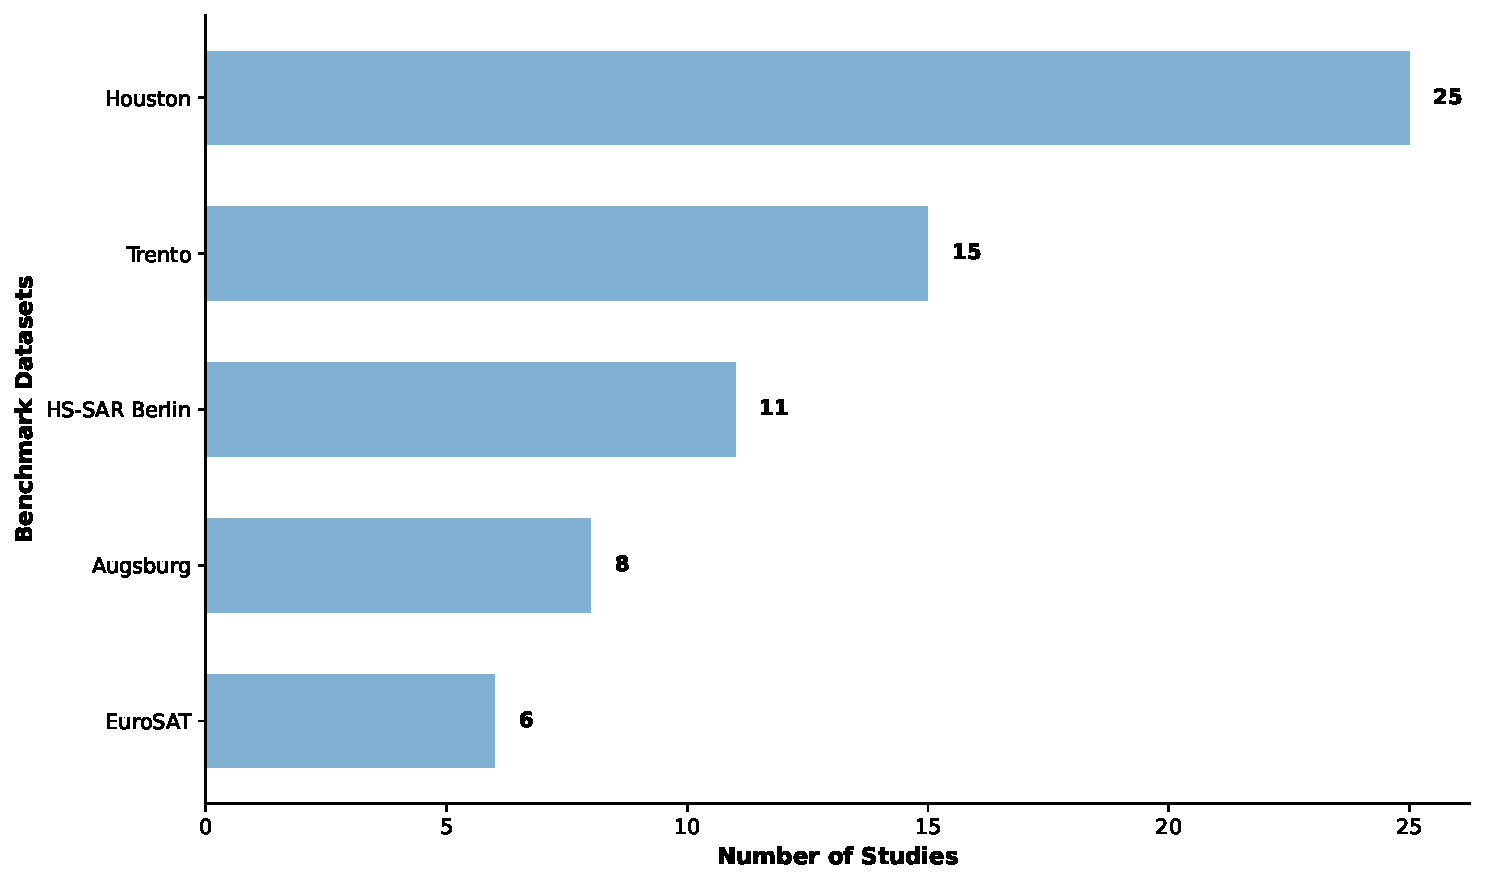
\includegraphics[width=0.85\columnwidth]{Figures/top_datasets_ranking.pdf}
	\caption{Frequency of benchmark datasets utilized in the analyzed LULC fusion studies.}
	\label{fig:datasets_ranking}
\end{figure}

% --- Table 4: 主要基准数据集技术规格 (严格对应柱状图中的前五个) ---
\begin{table}[!ht]
	\centering
	\setlength{\belowcaptionskip}{8pt}
	\caption{Technical specifications of the five most utilized benchmark datasets in LULC fusion research.}
	\label{tab:datasets_detail}
	\footnotesize
	\renewcommand{\arraystretch}{1.3}
	\begin{tabular}{@{} l l c c c @{}}
		\toprule
		\textbf{Dataset} & \textbf{Modalities (Sensors)} & \textbf{Resolution} & \textbf{Classes} & \textbf{Dimensions (px)} \\ 
		\midrule
		Houston 2013  & HSI (144 bands) + LiDAR      & 2.5 m   & 15 & $349 \times 1905$ \\ 
		Trento        & HSI (6 bands) + LiDAR        & 1.0 m   & 6  & $600 \times 166$ \\ 
		HS-SAR Berlin & HSI + SAR (dual-pol)         & 3.5 m   & 8  & $1623 \times 1076$ \\ 
		Augsburg      & SAR + HSI + DSM              & 30m / 1m & 7  & $1528 \times 918$ \\ 
		EuroSAT       & Multispectral (Sentinel-2)   & 10 m    & 10 & $64 \times 64$ (per patch) \\ 
		\bottomrule
	\end{tabular}
\end{table}

% --- 过渡段落：引出理论融合阶段 ---
As evidenced by the technical specifications in Table~\ref{tab:datasets_detail}, the integration of heterogeneous data requires different algorithmic strategies. The diversity in spatial resolution and spectral dimensionality across these benchmarks, particularly the HSI and LiDAR combinations in Houston and Muufl, has historically driven the evolution of fusion methodologies. 

Driven by this evidence, research typically categorizes fusion technologies into three progressive stages: Data-level Fusion, Feature-level Fusion, and Decision-level Fusion, as illustrated in Fig.~\ref{fig:fusion_stages}. The robust data structures provided by these benchmarks have specifically catalyzed the shift toward feature-level fusion, which uses deep learning to align complex semantic representations from different sensors.

\begin{figure}[!ht]
	\centering
	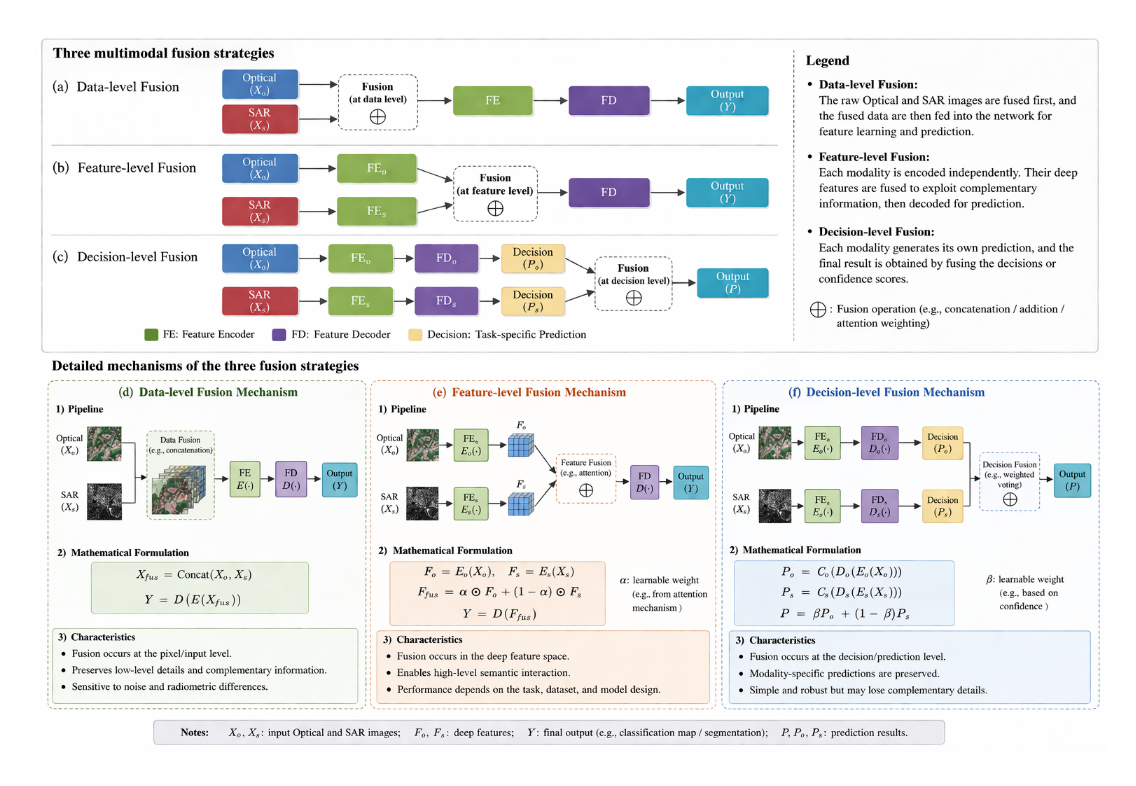
\includegraphics[width=1.0\columnwidth, trim=0 10 0 10, clip]{Figures/Fusion_Picture.pdf}
	\caption{Three stages of fusion technology in LULC: (a) data-level fusion, (b) feature-level fusion, and (c) decision-level fusion.}
	\label{fig:fusion_stages}
\end{figure}

\subsubsection{Data Fusion}
Data fusion, often referred to as pixel-level or raw-level fusion, involves the direct integration of multimodal data sources, such as optical imagery, LiDAR point clouds, and Synthetic Aperture Radar (SAR)\citep{57}. Bibliometric trends from 2016 to 2025 indicate that while keywords such as ``LiDAR'' and ``remote sensing'' maintain significant research heat \citep{38,39}, emerging focus has shifted toward the synergy of these sensors to overcome individual spectral or structural limitations. The prominent status of LiDAR is attributed to its capacity to provide high-precision 3D coordinates and vegetation structure information, which effectively compensates for the spectral saturation and cloud-cover vulnerabilities of optical sensors like Sentinel-2 \citep{40}.

Despite its foundational importance, data fusion faces persistent technical bottlenecks, particularly in multi-source spatial registration and heterogeneous noise suppression \citep{41}. Our analysis suggests a paradigm shift in the role of data fusion: it is no longer merely an end-to-end alignment task but has become an indispensable precursor for advanced feature-level modeling. High-quality fused inputs are now critical for empowering deep learning architectures ranging from local feature oriented CNN to global context aware Transformer and the more recent linear complexity Mamba models to achieve superior accuracy in complex LULC classification and simulation tasks. Consequently, the innovation in this domain is increasingly directed toward providing ``model-ready'' multimodal inputs that preserve both fine-grained textures and macro-scale spatial dependencies \citep{23,cao2020urban}.




% 请确保你在 main.tex 的导言区（\begin{document}之前）已经加上了这几行配置：
% \usepackage{booktabs}
% \usepackage{caption}
% \captionsetup[table]{labelfont=bf, textfont=it, labelsep=newline, justification=justified, singlelinecheck=false}

\begin{table}[htb!]
	\centering
	\setlength{\belowcaptionskip}{5pt}
	% 提示：配合导言区的 captionsetup，这里的标题会自动渲染为标准的 APA 换行+斜体格式
	\caption{Comparison of Deep Learning Models for Feature-level Fusion in LULC.}
	\label{tab:comparison_models}
	\footnotesize
	\renewcommand{\arraystretch}{1.4} % 稍微降低基础缩放，依靠 addlinespace 来提供自然的段落间隔
	\begin{tabular}{@{} p{1.8cm} p{2.8cm} p{3.3cm} p{3.1cm} p{3.5cm} @{}}
		\toprule
		\textbf{Method} & \textbf{Role in Fusion} & \textbf{Advantages} & \textbf{Disadvantages} & \textbf{Recent Trend} \\ 
		\midrule
		CNN \citep{2,8,29,56} & Backbone for local feature extraction. & Excels at texture/edge capture; fast convergence. & Limited receptive field; lacks global context. & Shifting toward Hybrid CNN-Transformer architectures. \\ 
		\addlinespace[0.8em] % 用优雅的空隙代替硬邦邦的内侧横线
		
		Transformer \citep{7,35,36,bazi2021vision,liu2024softformer} & Global feature interaction via self-attention. & Global receptive field; strong cross-modal interaction. & Quadratic complexity; high data demand. & Becoming the new SOTA; focus on efficient variants (Swin, SoftFormer). \\ 
		\addlinespace[0.8em]
		
		Attention Mechanisms \citep{46,47,zhang2023multimodal} & Adaptive weight regulation module. & Suppresses noise; enhances key features. & Increases computational overhead. & Evolving toward Cross-Modal Attention for spatial misalignment. \\ 
		\addlinespace[0.8em]
		
		Mamba \citep{5,49,53,he2024foundation} & Efficient sequence and global modeling. & Linear complexity; low memory consumption. & Early stage; lack of pre-trained models. & Development of Spatiotemporal frameworks (e.g., Geo-Mamba). \\ 
		\bottomrule
	\end{tabular}
\end{table}

\subsection{Feature-Level Fusion and Technical Evolution}

Feature-level fusion integrates abstract features at the intermediate layers of a model (such as feature maps extracted via CNN or Transformer), striking an optimal balance between information preservation and computational efficiency. Bibliometric analysis reveals that ``CNN'', ``deep learning'', and ``feature extraction'' are the highest-frequency keywords, alongside emerging terms such as ``Transformer'', ``attention mechanism'', ``representation learning'', and ``semantic segmentation''.

% 完整修改后的代码（方案二）
Deep Learning (DL): As the foundation of the modern technical ecosystem, DL provides an end-to-end framework for feature-level fusion, enabling the unified implementation of automated feature extraction and decision-making. In LULC research, DL models automatically mine multi-dimensional spectral, spatial, and textural features, overcoming the bottlenecks of manual feature engineering. This has established feature-level fusion as a mainstream strategy \citep{42,43}. Notably, the study ``Deep Learning Earth Observation Classification Using ImageNet Pretrained Networks'' \citep{28} has reached a TGCS of 492, reflecting the intense research focus on DL-driven methodologies.

\medskip % 增加段落间距
CNN (Convolutional Neural Network): CNN served as the core tools for early feature-level fusion. They excel at capturing local spatial features, such as building textures and vegetation patch structures. By extracting and fusing local features from multi-source data (e.g., optical and SAR) through channel concatenation or weighted summation, CNN significantly enhance classification accuracy in complex heterogeneous surfaces \citep{41}.

\medskip
Transformer: This architecture has seen a rapid surge in popularity. In 2023, the study ``Extended Vision Transformer (ExViT) for Land Use and Land Cover Classification'' \citep{36} achieved a TGCS of 312. By utilizing self-attention mechanisms, Transformer transcend the local receptive field limitations of CNN, capturing long-range spatial dependencies such as large-scale urban expansion patterns and watershed-scale connectivity \citep{45}.

\medskip
Feature Extraction and Attention Mechanisms: These represent the core technical phases of fusion. Feature extraction is the prerequisite, converting raw multi-source data (optical, SAR, LiDAR) into discriminative abstract representations. Meanwhile, the attention mechanism acts as an intelligent regulator, automatically learning weights to prioritize features most relevant to LULC tasks, such as building edges or specific vegetation signatures \citep{46,47}.

\medskip
Semantic Segmentation: This is the most prevalent application scenario for feature fusion. LULC research requires not only type identification but also the precise delineation of spatial boundaries. By integrating complementary information, feature fusion produces refined segmentation results for roads, buildings, and green spaces, meeting the demand for ``precision geoscience'' \citep{45,48}.

Of particular note is the rapid emergence of the \textbf{Mamba} architecture. Although it currently appears with low frequency (only 4 times) in the keyword co-occurrence network \citep{49,5,51,52}, it is positioning itself as the next-generation backbone following CNN and Transformer. While Transformer possess superior global modeling capabilities, their computational complexity grows quadratically with image resolution. In contrast, Mamba introduces a \textit{Selective Scan} mechanism \citep{53}, achieving a global receptive field with linear complexity. Recent studies, such as ``Geo-Mamba'' \citep{49} and ``Semi-Mamba'' \citep{51}, illustrate Mamba's potential in breaking the accuracy-efficiency bottleneck. However, as an architecture proposed in late 2023, its application in LULC remains in its infancy and requires further empirical validation.

In summary, feature-level fusion has developed into diverse technical lineages. To clearly illustrate the positioning and evolution of different deep learning architectures, Table~\ref{tab:comparison_models} compares the characteristics of mainstream models and key components. The technical focus is shifting from local-centric CNN toward global-centric Transformer and efficiency-oriented architectures like Mamba.



\subsubsection{Decision-level Fusion}
Decision-level fusion, also known as late fusion, represents a high-level integration strategy where independent classification or simulation outputs from multiple sub-models are combined to reach a final consensus \citep{ORIGPu2023DecisionFusion}. Bibliometric data identifies keywords such as ensemble learning, ``Random Forest'', and ``voting strategies'' as the primary methodological pillars of this stage \citep{55}. Despite its foundational role in traditional machine learning, our analysis shows that its research heat in the LULC domain has remained relatively low compared to feature-level approaches.

The primary limitation of decision-level fusion lies in its ``information decoupling'' nature: by processing each data source independently, it often fails to capture the intricate, deep-level complementary relationships and cross-modal correlations inherent in multi-source datasets \citep{ORIG6}. This can lead to a loss of fine-grained spatial-spectral dependencies, resulting in lower overall accuracy and a lack of interpretability regarding the underlying driving mechanisms of LULC changes. However, recent trends suggest a niche resurgence of decision-level fusion in scenarios requiring high model reliability. By leveraging diverse architectures, such as combining the local spatial biases of CNN with the global dependencies of Transformer \citep{bazi2021vision}, decision fusion acts as a robust ensemble layer that mitigates the risk of single-model over-fitting \citep{belgiu2016random}. Thus, while no longer the primary driver of algorithmic speed, it remains a critical tool for uncertainty estimation and multi-model verification in high-precision LULC tasks.
%\FloatBarrier



\section{Challenges in LULC Studies}
Based on the bibliometric analysis, a distinct contrast emerges: while algorithmic keywords such as \textit{Deep Learning}, \textit{Transformer}, and \textit{Fusion} exhibit extremely high heat, terms related to \textit{Data Quality}, \textit{Uncertainty Analysis}, and \textit{Error Propagation} remain relatively marginalized. This suggests that current research emphasis leans heavily toward architectural innovation, potentially overlooking the reliability of the underlying data. In LULC studies, data reliability is paramount; it serves as the foundation for deep learning models. However, the acquisition and integration of high-quality data still face severe challenges.

\subsection{Data-Level Challenges}

In the following, we categorize the challenges associated to the data in three aspects:

\begin{enumerate}
	\item \textbf{Intrinsic Quality and Uncertainty:} Raw data quality is a persistent issue. Optical imagery is frequently obscured by cloud cover and lighting variations; SAR imagery suffers from inherent speckle noise; and LiDAR point clouds often contain outliers. Deep learning models, particularly Transformer, are highly sensitive to noise, and errors in raw data can be amplified during feature extraction, leading to distorted classification results.
	\item \textbf{Spatiotemporal Inconsistency:} This represents a core physical barrier to effective fusion. Optical, SAR, and LiDAR data possess natural discrepancies in spatial resolution, observation angles, and imaging times. Existing registration algorithms struggle to eliminate sub-pixel offsets, and such spatial misalignments can lead models to learn incorrect feature correspondences. Furthermore, radiometric drift in long-term monitoring may trigger ``pseudo-change'' misinterpretations.
	\item \textbf{Scarcity of High-Quality Annotations:} The development of supervised learning is bottlenecked by the lack of labeled samples \citep{56}. LULC tasks require precise pixel-level annotation, which demands extensive expert knowledge and is time-consuming. In complex mixed-pixel regions, subjective inconsistencies in manual labeling can lead to model overfitting, limiting applications in large-scale scenarios.
\end{enumerate}





\subsection{Algorithm-Level Challenges}

In the following, we categorize the challenges associated with algorithms into three aspects, setting the stage for the subsequent discussion of potential remedies.


\begin{enumerate}
	\item \textbf{Semantic Gap in Multi-modal Features:} There is a significant distribution difference between the spectral features (chemical attributes) of optical imagery and the structural features (physical attributes) of SAR/LiDAR. Current mainstream fusion methods, such as simple channel concatenation or weighted summation, lack adaptive feature alignment mechanisms. This makes it difficult to fully exploit the complementarity between heterogeneous data, resulting in the loss of critical information.
	
	\item \textbf{Lack of Interpretability:} Despite their high accuracy, CNN and Transformer are often viewed as black boxes. It is difficult to intuitively reveal the physical mechanisms behind classification decisions, for instance, whether the model relies on LiDAR height info or optical texture. This opacity makes it challenging to quantify the contribution of different driving factors to LULC changes, weakening the persuasiveness of geographical explanations.
	
	\item \textbf{Insufficient Generalization:} Most existing models follow the ``Independent and Identically Distributed'' (IID) assumption. However, real-world LULC scenarios (e.g., from urban to mountainous areas) exhibit significant \textit{Domain Shift}. Models trained in specific regions often suffer performance degradation when migrated to heterogeneous new areas or time periods, hindering the goal of ``train once, apply globally''. 
\end{enumerate}



\section{Conclusion}
Based on the Web of Science Core Collection, this study utilizes bibliometric and network analysis methods to systematically review the application of deep learning (DL) and multi-source data fusion in LULC simulation from 2006 to 2025. Analysis of 261 core publications reveals that since 2016, research activity has grown exponentially, marking a decisive shift in the methodological landscape. Deep learning has thoroughly replaced traditional machine learning,such as SVM and Random Forest as the dominant paradigm, demonstrating superior performance in handling the complexities of remote sensing big data. From a global perspective, China and Germany have emerged as the primary hubs of innovation, leading in both publication volume and long-term citation impact.

The technical evolution analyzed in this review underscores a fundamental transition from single-source data processing to heterogeneous multi-source fusion. Feature-level fusion, which leverages sophisticated neural architectures to integrate the complementary spectral, structural, and textural information from optical imagery, SAR, and LiDAR, has established itself as the most robust and versatile strategy. We observed a clear evolutionary trajectory: the field is rapidly moving from the local feature centric approach of CNN to global context aware modeling enabled by Transformer and attention mechanisms. Furthermore, the emergence of State Space Models (e.g., Mamba) hints at a future shift toward architectures that balance high-order spatial modeling with linear computational efficiency.

However, the transition to ``Deep Fusion'' is not without critical bottlenecks. Despite achieving record-breaking classification accuracies, significant challenges remain regarding data reliability and model robustness. The spatiotemporal inconsistencies between multi-modal sensors continue to introduce ``pseudo-changes'' in simulation results. Moreover, the ``black box'' nature of current state-of-the-art models limits their utility in decision-making processes where geographical interpretability is essential. The high dependence on massive labeled datasets also hinders the generalization of these models to regions where ground-truth data is scarce.

Looking forward, this study identifies three critical directions for future LULC research. First, the integration of Explainable Artificial Intelligence (XAI) is paramount. Future frameworks must move beyond black box predictions. Incorporating XAI into multi-source fusion models will allow researchers to quantify the specific contributions of various features, thereby bridging the current gap between deep learning outputs and traditional geographical process understanding. Second, there is an urgent need for General Remote Sensing Foundation Models. To address the persistent scarcity of high-quality ground truth annotations, developing large-scale foundation models that can be effectively fine-tuned via few-shot or zero-shot learning will be essential for achieving robust global scale monitoring. Third, advancing Intelligent Data Governance and Harmonization remains a core technical requirement. Advanced registration and normalization algorithms are needed to resolve the physical discrepancies between heterogeneous sensors. This ensures that multi-source fusion occurs on ``model-ready'' data that preserves critical fine-grained textures while eliminating spatiotemporal noise.

In summary, the integration of deep learning and multi-source fusion has opened a new era for LULC research. While the field has made remarkable strides in technical complexity, future breakthroughs will depend on a holistic balance between model accuracy, physical interpretability, and cross scene generalization. Such advancements will provide more reliable, evidence-based scientific support for global environmental monitoring and sustainable land resource management.


\bibliographystyle{apacite}
\bibliography{interactapasample}

\end{document}
